\documentclass[12pt,a4paper]{article}

% Package imports
\usepackage[utf8]{inputenc}
\usepackage[T1]{fontenc}
\usepackage{geometry}
\usepackage{graphicx}
\usepackage{booktabs}
\usepackage{longtable}
\usepackage{array}
\usepackage{multirow}
\usepackage{hyperref}
\usepackage{natbib}
\usepackage{float}
\usepackage{caption}
\usepackage{subcaption}
\usepackage{xcolor}
\usepackage{setspace}

% Page geometry
\geometry{
    a4paper,
    total={170mm,257mm},
    left=20mm,
    top=20mm,
}

% Hyperlink setup
\hypersetup{
    colorlinks=true,
    linkcolor=blue,
    filecolor=magenta,
    urlcolor=cyan,
    citecolor=blue,
}

% Line spacing
\onehalfspacing

% Title information
\title{\textbf{Financial Accounting Analysis of Apple Inc.:}\\
\textbf{Performance Assessment and Strategic Insights Through Ratio Analysis}}
\author{Financial Accounting Research Project}
\date{January 2025}

\begin{document}

\maketitle

\tableofcontents
\newpage

% =============================================================================
% SECTION 1: INTRODUCTION TO THE ORGANISATION
% =============================================================================
\section{Introduction to the Organisation}

\subsection{Organisational Background and Business Model}

Apple Inc. is a multinational technology corporation headquartered in Cupertino, California, United States. Founded in April 1976 by Steve Jobs, Steve Wozniak, and Ronald Wayne, the organisation has evolved from a garage-based computer manufacturer into the world's largest publicly traded corporation by market capitalisation. As of 2024, Apple's market capitalisation exceeded \$3 trillion, reflecting its position as the most valuable company globally \citep{apple202410k}.

\paragraph{Business Model and Product Ecosystem}

Apple's business model is founded on an integrated ecosystem of hardware, software, and services designed to create customer loyalty and recurring revenue streams. The organisation's product portfolio comprises five principal categories: (1) iPhone smartphones, which remain the largest revenue generator; (2) Mac personal computers including MacBook, iMac, and Mac Pro; (3) iPad tablets; (4) wearables and home accessories comprising Apple Watch, AirPods, and Apple TV; and (5) services including the App Store, Apple Music, Apple TV+, Apple Arcade, iCloud, Apple Pay, and Apple Care \citep{apple202410k}.

The services division has emerged as a critical growth driver, with revenue increasing from \$85.2 billion in 2023 to \$96.2 billion in 2024, representing 24.6\% of total net sales. This shift toward services revenue is strategically significant as services carry higher gross margins (approximately 70\%) compared to hardware products (approximately 35-40\%), thereby improving overall profitability whilst reducing dependence on iPhone upgrade cycles \citep{apple202410k}.

\paragraph{Competitive Positioning and Market Dynamics}

Apple maintains competitive advantages through several strategic pillars: (1) brand equity and customer loyalty; (2) proprietary operating systems (iOS, macOS, watchOS, tvOS); (3) vertical integration controlling both hardware and software; (4) the App Store ecosystem with over 2 million applications; and (5) premium positioning enabling superior profit margins relative to competitors \citep{kieso2023}.

The organisation operates in highly competitive technology markets, facing rivalry from Samsung Electronics (smartphones), Microsoft and Dell (personal computers), Google (mobile operating systems and cloud services), and Amazon and Netflix (digital streaming). Despite this competition, Apple maintains pricing power through product differentiation, ecosystem lock-in, and perceived quality advantages \citep{brealey2020}.

\paragraph{Geographic Operations and Organisational Scale}

Geographically, Apple operates through five reportable segments: Americas (United States, Canada, and Latin America), Europe, Greater China, Japan, and Rest of Asia Pacific. International markets accounted for 61.8\% of total net sales in 2024, demonstrating the organisation's global reach. The Greater China region, comprising mainland China, Hong Kong, and Taiwan, represents the largest international market, generating \$65.1 billion in revenue during 2024 \citep{apple202410k}.

As of September 28, 2024, the organisation employed approximately 164,000 full-time equivalent personnel worldwide across retail stores, corporate offices, research and development facilities, and manufacturing operations. This scale necessitates sophisticated financial management systems to coordinate operations across multiple jurisdictions, tax environments, and regulatory regimes \citep{apple202410k}.

\paragraph{Supply Chain and Manufacturing Operations}

Apple does not manufacture products internally but relies on a global network of contract manufacturers, primarily Foxconn (Hon Hai Precision Industry), Pegatron, and TSMC (Taiwan Semiconductor Manufacturing Company). This outsourcing model enables capital efficiency whilst requiring rigorous supplier quality management and financial controls. The organisation's supply chain spans multiple continents, with significant manufacturing concentration in China, Vietnam, and India \citep{apple202410k}.

The organisation maintains substantial inventory despite the outsourcing model, with inventory balances of \$7.286 billion as of September 28, 2024. This inventory level, whilst material, represents exceptional efficiency with an inventory turnover ratio of 53.67 times, indicating that inventory is sold and replenished approximately every 6.8 days \citep{apple202410k}.

\paragraph{Financial Scale and Capital Structure}

The organisation's shares are traded on the NASDAQ stock exchange under the ticker symbol AAPL. Apple is a component of major stock indices including the Dow Jones Industrial Average, S\&P 500, and NASDAQ-100. For the fiscal year ended September 28, 2024, Apple reported total net sales of \$391.035 billion, representing a 2.0\% increase from \$383.285 billion in fiscal year 2023 \citep{apple202410k}.

Apple's capital structure is characterised by substantial financial leverage, with total debt of \$96.662 billion offset by \$65.171 billion in cash and marketable securities, resulting in net debt of \$31.491 billion. The organisation employs debt strategically to fund capital returns to shareholders through share repurchases and dividends, having returned \$110.2 billion to shareholders in 2024 (\$95.0 billion in repurchases and \$15.2 billion in dividends) \citep{apple202410k}.

\subsection{Importance of Financial Accounting for Apple Inc.}

Financial accounting serves as the indispensable foundation for Apple's strategic decision-making, capital allocation, and stakeholder communication processes. Given the organisation's scale, global operations, and complex business model, accurate financial reporting is essential for multiple critical dimensions of corporate governance and value creation.

\paragraph{Regulatory Compliance and Public Trust}

As a publicly traded corporation listed on the NASDAQ exchange, Apple is subject to extensive regulatory reporting requirements established by the US Securities and Exchange Commission (SEC). The organisation must prepare financial statements in accordance with US Generally Accepted Accounting Principles (GAAP), as established by the Financial Accounting Standards Board (FASB), and file comprehensive reports including the annual Form 10-K, quarterly Form 10-Q, and current reports on Form 8-K \citep{fasb2024, sec2024}. These regulatory filings provide transparency to investors, analysts, regulators, and the public regarding the organisation's financial position, performance, and risk factors.

The Sarbanes-Oxley Act of 2002 imposes additional requirements, including Section 404 which mandates management assessment and external auditor attestation of internal control effectiveness \citep{sox2002}. Compliance with these requirements demands significant investment in financial systems, internal audit functions, and disclosure controls. Apple's financial statements are audited annually by Ernst \& Young LLP, one of the ``Big Four'' public accounting firms, providing independent verification of financial reporting reliability \citep{apple202410k}.

\paragraph{Capital Market Communication and Valuation}

Apple's market capitalisation exceeding \$3 trillion reflects investor confidence based substantially on reported financial results. Investment decisions by institutional investors, pension funds, mutual funds, and individual retail investors rely heavily on the organisation's financial statements. The stock price responds directly to reported quarterly earnings, revenue growth rates, profit margins, and forward-looking guidance provided by management \citep{brealey2020}.

Financial accounting information enables equity analysts to construct valuation models, project future cash flows, and make buy, sell, or hold recommendations. Accurate and timely financial reporting ensures that the capital markets receive complete information for efficient capital allocation. The organisation's price-to-earnings ratio, enterprise value, and other valuation multiples are derived directly from reported financial metrics \citep{kieso2023}.

\paragraph{Strategic Decision-Making and Performance Measurement}

Apple's management utilises financial accounting information for critical strategic decisions across multiple dimensions. The organisation invested \$31.370 billion in research and development during fiscal year 2024, representing 8.0\% of net sales, requiring accurate cost accounting to evaluate project profitability and allocate resources across iPhone, Mac, iPad, wearables, and services development initiatives \citep{apple202410k}.

Segment reporting for five geographic regions (Americas, Europe, Greater China, Japan, and Rest of Asia Pacific) enables management to assess regional performance, identify growth opportunities, and allocate marketing and distribution resources effectively. Each geographic segment's revenue, operating income, and assets are tracked separately, facilitating performance evaluation and strategic planning \citep{apple202410k}.

\paragraph{Capital Structure Management and Shareholder Returns}

The organisation's substantial capital return programme, which totalled \$110.2 billion in 2024 (\$95.0 billion in share repurchases and \$15.2 billion in dividends), requires rigorous financial accounting to determine appropriate levels of capital distribution whilst maintaining financial flexibility for operations, acquisitions, and investments \citep{apple202410k}.

Financial accounting information enables treasury and finance teams to monitor debt compliance covenants, assess borrowing capacity, and optimise the capital structure between debt and equity financing. The organisation's debt-to-equity ratio of 1.70 reflects a deliberate strategy of employing low-cost debt to fund share repurchases, thereby enhancing earnings per share and return on equity metrics whilst maintaining investment-grade credit ratings \citep{apple202410k}.

\paragraph{Supply Chain Management and Operational Efficiency}

Financial accounting information supports operational excellence across Apple's global supply chain. The organisation tracks inventory levels, accounts payable to suppliers, and accounts receivable from distributors and carriers to optimise working capital management. The exceptional inventory turnover ratio of 53.67 times indicates world-class supply chain coordination that depends on accurate cost accounting and inventory valuation \citep{apple202410k}.

Product profitability analysis enables pricing decisions, portfolio management, and investment prioritisation. The gross margin differential between products (iPhone approximately 45-50\%, services approximately 70\%) informs strategic emphasis toward higher-margin offerings. This level of financial insight requires sophisticated cost allocation methodologies and accurate revenue recognition practices \citep{kieso2023}.

% =============================================================================
% SECTION 2: UNDERSTANDING FINANCIAL ACCOUNTING IN THE BUSINESS
% =============================================================================
\section{Understanding Financial Accounting in the Business}

\subsection{Accounting Processes and Information Systems}

Apple's financial accounting function operates within a sophisticated enterprise resource planning (ERP) framework designed to ensure accuracy, timeliness, compliance, and transparency in financial reporting across global operations. The organisation prepares consolidated financial statements in accordance with US GAAP, which encompasses standards issued by the Financial Accounting Standards Board (FASB) and regulations enforced by the Securities and Exchange Commission (SEC) \citep{fasb2024}.

\paragraph{Accounting Cycle and Recording Processes}

The accounting cycle at Apple encompasses the systematic process of recording, classifying, and summarising financial transactions. The cycle commences with transaction identification, wherein economic events such as product sales, supplier payments, employee compensation, and borrowing activities are recognised and recorded in the organisation's accounting information system. Transactions are initially documented through source documents including sales invoices, purchase orders, supplier invoices, payroll records, and bank statements \citep{kieso2023}.

Journal entries are prepared to record transactions in the organisation's general ledger, applying the double-entry bookkeeping system wherein each transaction affects at least two accounts through debits and credits of equal amounts. For example, a product sale on credit generates a journal entry debiting accounts receivable and crediting sales revenue for the invoice amount, simultaneously recording cost of goods sold by debiting that expense account and crediting inventory \citep{kieso2023}.

Apple's accounting system processes millions of transactions daily across multiple business units and geographic regions. Sales transactions from Apple Stores, online stores, and distributor channels are recorded continuously throughout each day. Accounts payable records supplier invoices for components, manufacturing services, and operational expenditures. Accounts receivable tracks amounts owed by distributors, carriers, and enterprise customers \citep{apple202410k}.

\paragraph{Period-End Accounting Procedures}

At the conclusion of each fiscal quarter, comprehensive period-end accounting procedures are executed to ensure accurate financial reporting. These procedures encompass accrual adjustments wherein expenses incurred but not yet paid are recorded (such as accrued wages, interest expense, and warranty obligations), and revenue earned but not yet recorded is recognised \citep{kieso2023}.

Deferred revenue accounting is particularly significant for Apple's business model. When customers purchase devices, the organisation allocates a portion of the transaction price to deferred revenue to recognise the value of bundled services including Apple Music, Apple TV+, iCloud storage, and Apple Care protection plans over the expected service delivery period. This allocation requires judgment regarding estimated customer adoption rates and service life assumptions \citep{apple202410k}.

Inventory valuation requires periodic physical counts and cycle counting procedures to verify recorded quantities against actual physical inventory at manufacturing facilities, warehouses, and retail stores. Inventory is valued at the lower of cost or net realisable value, with cost determined using the first-in, first-out (FIFO) method, which assumes that the earliest inventory acquired is the first inventory sold \citep{apple202410k}.

\paragraph{Accounting Estimates and Judgments}

The preparation of Apple's financial statements requires management to make estimates, assumptions, and judgments that affect reported amounts. Critical accounting estimates include product warranty obligations, wherein the organisation estimates the expected cost of future warranty claims based on historical experience and product-specific failure rates. As of September 28, 2024, Apple's warranty liability stood at \$9.988 billion \citep{apple202410k}.

Income tax provisions require complex calculations involving multiple jurisdictions with varying tax rates, temporary differences from book and tax depreciation methods, and uncertain tax positions subject to challenge by tax authorities. The organisation recorded a provision for income taxes of \$21.541 billion in 2024, including the \$10.2 billion charge related to the European Commission State Aid Decision \citep{apple202410k}.

Fair value measurements for marketable securities and other financial instruments require estimation using appropriate valuation techniques. Level 2 fair value measurements for corporate securities utilise observable market inputs, whilst Level 3 measurements for certain private investments require management judgment and estimation techniques \citep{fasb2024}.

\paragraph{Internal Control Environment}

Apple maintains robust internal controls over financial reporting, as mandated by the Sarbanes-Oxley Act of 2002, to ensure the reliability of financial information \citep{sox2002}. Section 404 of the Act requires management to assess and report on the effectiveness of internal control over financial reporting, and for the organisation's independent auditor to attest to management's assessment.

The internal control environment encompasses control activities including: (1) segregation of duties wherein transaction initiation, recording, and reconciliation responsibilities are assigned to separate individuals; (2) authorization limits requiring management approval for material transactions; (3) physical safeguards protecting assets from unauthorised access or misappropriation; (4) reconciliations comparing recorded amounts to independent external records such as bank statements and supplier statements; and (5) information technology controls restricting system access and maintaining audit trails of system modifications \citep{kieso2023}.

Apple's internal audit function independently evaluates the effectiveness of internal controls, identifies control deficiencies, and recommends improvements to management and the Audit Committee of the Board of Directors. The organisation's disclosure controls and procedures ensure that information required to be disclosed in SEC filings is recorded, processed, summarised, and reported within specified time periods \citep{apple202410k}.

\paragraph{Independent Audit and Assurance}

Ernst \& Young LLP, an independent registered public accounting firm and one of the ``Big Four'' accounting firms, audits Apple's financial statements annually. The audit examination encompasses planning, risk assessment, internal control testing, substantive transaction testing, and confirmation procedures with external parties including customers, suppliers, and financial institutions \citep{apple202410k}.

The audit opinion issued by Ernst \& Young provides reasonable assurance that the financial statements present fairly, in all material respects, the financial position, results of operations, and cash flows of Apple Inc. in conformity with US GAAP. This independent verification enhances the credibility of financial information presented to investors, lenders, regulators, and other stakeholders \citep{kieso2023}.

\subsection{Main Financial Statements and Their Purposes}

Apple's financial reporting framework comprises three primary financial statements that provide complementary perspectives on the organisation's financial position, performance, and cash flows. These statements are prepared in accordance with US GAAP and are audited annually by independent registered public accountants \citep{fasb2024}.

\subsubsection{Consolidated Statements of Operations}

The Consolidated Statements of Operations, also referred to as the profit and loss statement, presents Apple's revenues, expenses, and profitability over specific accounting periods (typically fiscal years and quarters). This statement is fundamental for assessing the organisation's ability to generate profits from its core operations, evaluate revenue growth trends, and understand cost structure dynamics \citep{kieso2023}.

\begin{table}[H]
\centering
\caption{Consolidated Statements of Operations Summary (Fiscal Years 2023-2024)}
\label{tab:operations_summary}
\begin{tabular}{lrrr}
\toprule
\textbf{Item} & \textbf{2024 (\$ millions)} & \textbf{2023 (\$ millions)} & \textbf{Change (\%)} \\
\midrule
Total net sales & 391,035 & 383,285 & +2.0\% \\
Cost of sales & 210,352 & 214,137 & -1.8\% \\
Gross margin & 180,683 & 169,148 & +6.8\% \\
Operating income & 123,216 & 114,301 & +7.8\% \\
Net income & 93,736 & 96,995 & -3.4\% \\
\bottomrule
\end{tabular}
\end{table}

As indicated in Table~\ref{tab:operations_summary}, the organisation achieved \$391.035 billion in net sales during fiscal year 2024, representing a 2.0\% increase from the prior year. Gross margin improved to \$180.683 billion, yielding a gross profit margin of 46.21\%. However, net income decreased by 3.4\% to \$93.736 billion, primarily resulting from a one-time income tax charge of \$10.2 billion related to the European Commission's State Aid Decision \citep{apple202410k}.

\paragraph{Statement Structure and Key Components}

The statement of operations follows a multi-step format that separates operating performance from non-operating items. Net sales represent revenue from product sales and services after deducting returns, allowances, and discounts. Cost of sales encompasses direct costs including manufacturing expenses, component costs, freight, and warranty expenses. Gross margin, calculated as net sales minus cost of sales, indicates the profitability of core products before operating expenses \citep{kieso2023}.

Operating expenses include research and development expenses (\$31.370 billion in 2024) reflecting investment in new products and technologies, and selling, general and administrative expenses (\$26.097 billion in 2024) covering retail operations, marketing, corporate overhead, and executive compensation. Operating income represents profit from core business operations before interest and taxes \citep{apple202410k}.

Other income and expense includes interest income, interest expense, and non-recurring items. Provision for income taxes represents current and deferred tax obligations. Net income, the bottom-line profit figure, is available for distribution to shareholders or retention for business operations. Earnings per share calculations divide net income by weighted-average shares outstanding, with basic EPS using actual shares outstanding and diluted EPS assuming conversion of potentially dilutive securities \citep{kieso2023}.

\subsubsection{Consolidated Balance Sheets}

The Consolidated Balance Sheets present a snapshot of Apple's financial position at specific points in time (typically quarter-end and year-end dates). Following the fundamental accounting equation wherein Assets equals Liabilities plus Shareholders' Equity, this statement is essential for assessing the organisation's liquidity, solvency, capital structure, and financial flexibility \citep{kieso2023}.

\begin{table}[H]
\centering
\caption{Consolidated Balance Sheets Summary (as of September 28, 2024 and September 30, 2023)}
\label{tab:balance_sheet_summary}
\begin{tabular}{lrr}
\toprule
\textbf{Item} & \textbf{2024 (\$ millions)} & \textbf{2023 (\$ millions)} \\
\midrule
\textbf{Assets} \\
Cash and cash equivalents & 29,943 & 29,965 \\
Marketable securities & 126,707 & 132,134 \\
Accounts receivable, net & 33,410 & 29,508 \\
Inventories & 7,286 & 6,331 \\
Total current assets & 152,987 & 143,566 \\
Total assets & 364,980 & 352,583 \\
\midrule
\textbf{Liabilities and Shareholders' Equity} \\
Accounts payable & 68,960 & 62,611 \\
Commercial paper & 9,967 & 5,985 \\
Term debt (current portion) & 10,912 & 9,822 \\
Total current liabilities & 176,392 & 145,308 \\
Total liabilities & 308,030 & 290,437 \\
Total shareholders' equity & 56,950 & 62,146 \\
\bottomrule
\end{tabular}
\end{table}

As shown in Table~\ref{tab:balance_sheet_summary}, the organisation held total assets of \$364.980 billion as of September 28, 2024, comprising current assets of \$152.987 billion and non-current assets of \$211.993 billion. Total liabilities of \$308.030 billion included current liabilities of \$176.392 billion and long-term debt of \$85.750 billion \citep{apple202410k}.

\paragraph{Asset Classification and Composition}

Assets are classified as current if expected to be realised or consumed within one year, or non-current if expected to provide benefits beyond one year. Current assets (\$152.987 billion in 2024) include cash and cash equivalents (\$29.943 billion) representing immediately available funds; marketable securities (\$126.707 billion) comprising highly liquid debt and equity securities; accounts receivable (\$33.410 billion) representing amounts owed by customers; inventory (\$7.286 billion) comprising components and finished goods; and other current assets including vendor non-receivables and deferred tax assets \citep{apple202410k}.

Non-current assets (\$211.993 billion) include marketable securities (\$100.288 billion) with longer maturities; property, plant and equipment (\$50.963 billion) comprising manufacturing facilities, retail stores, corporate offices, and equipment; and other non-current assets including intangible assets, goodwill, and deferred tax assets. Property, plant and equipment are recorded at cost less accumulated depreciation, with depreciation expense recognised systematically over the estimated useful lives of the assets \citep{kieso2023}.

\paragraph{Liability Classification and Composition}

Liabilities are classified as current if due within one year, or non-current if due after one year. Current liabilities (\$176.392 billion in 2024) include accounts payable (\$68.960 billion) representing amounts owed to suppliers for components and manufacturing services; commercial paper (\$9.967 billion) and term debt (\$10.912 billion) representing short-term borrowings; and other current liabilities including accrued expenses and deferred revenue \citep{apple202410k}.

Non-current liabilities (\$131.638 billion) include term debt (\$85.750 billion) comprising fixed-rate borrowings with maturities extending beyond one year; and other non-current liabilities including deferred tax liabilities and other long-term obligations. The organisation's debt portfolio includes various fixed-rate notes issued in multiple currencies, with interest rates ranging from approximately 0.5\% to 4.7\% and maturities extending through 2052 \citep{apple202410k}.

\paragraph{Shareholders' Equity Components}

Total shareholders' equity (\$56.950 billion in 2024) represents the residual interest in assets after deducting liabilities. The principal components include common stock (\$74.813 billion at par value) and retained earnings (-\$1.351 billion), with additional paid-in capital reflecting amounts received from shareholders above par value. The deficit in retained earnings reflects accumulated comprehensive losses and substantial dividends and share repurchases that have exceeded cumulative net income over recent periods \citep{apple202410k}.

\subsubsection{Consolidated Statements of Cash Flows}

The Consolidated Statements of Cash Flows track cash inflows and outflows across three categories: operating activities, investing activities, and financing activities. This statement is essential for assessing the organisation's ability to generate cash from operations, fund investments, and meet financing obligations. Unlike the statement of operations which follows accrual accounting, the cash flow statement presents actual cash movements during the period \citep{kieso2023}.

\paragraph{Operating Activities}

Cash flows from operating activities represent cash generated from core business operations. Apple utilises the indirect method, commencing with net income (\$93.736 billion in 2024) and making adjustments for non-cash items including depreciation, amortisation, share-based compensation expense, and deferred income tax expense. Changes in working capital accounts are then added or subtracted: increases in operating assets (such as accounts receivable and inventory) represent cash outflows, whilst increases in operating liabilities (such as accounts payable and deferred revenue) represent cash inflows \citep{apple202410k}.

In 2024, Apple generated \$118.254 billion in cash from operating activities, substantially exceeding the \$99.586 billion generated in 2023. This 18.8\% increase reflects improved earnings quality and efficient working capital management. The operating cash flow to net income ratio of 126.2\% (\$118.254 billion divided by \$93.736 billion) indicates strong earnings conversion to cash \citep{apple202410k}.

\paragraph{Investing Activities}

Cash flows from investing activities represent cash used for or generated from investments in long-term assets and marketable securities. In 2024, Apple used \$52.790 billion for purchases of marketable securities and received \$57.972 billion from maturities and sales of marketable securities, resulting in net cash provided by investing activities of \$2.935 billion. Capital expenditures (property, plant and equipment additions) consumed \$11.053 billion, reflecting ongoing investment in retail stores, data centers, and corporate infrastructure \citep{apple202410k}.

\paragraph{Financing Activities}

Cash flows from financing activities represent cash transactions with providers of capital and distributions to shareholders. In 2024, Apple used \$121.983 billion for financing activities, comprising \$95.015 billion for share repurchases, \$15.233 billion for dividends and dividend equivalents, and \$12.641 billion for net debt repayments. These capital return activities substantially exceeded the proceeds from debt issuance and employee stock plan exercises, resulting in significant net cash outflow \citep{apple202410k}.

\subsection{Key Accounting Policies and Their Application}

Apple's financial statements reflect application of significant accounting policies that govern revenue recognition, inventory valuation, asset measurement, and financial instrument presentation. These policies, selected by management and applied consistently, materially affect the reported financial results and position \citep{kieso2023}.

\paragraph{Revenue Recognition Policy}

Apple recognises revenue in accordance with Accounting Standards Codification (ASC) Topic 606, \textit{Revenue from Contracts with Customers}, which requires revenue to be recognised when (or as) the organisation satisfies a performance obligation by transferring control of promised goods or services to a customer \citep{fasb2014}. The amount of revenue recognised reflects the consideration to which the organisation expects to be entitled in exchange for transferring goods or services.

For hardware products including iPhone, Mac, iPad, and wearables, revenue is typically recognised upon shipment to customers, as this represents the point at which control transfers and performance obligations are satisfied. For products sold through Apple Stores, revenue is recognised at the time of sale. For products sold through distribution channels or carriers, revenue recognition may be delayed depending on specific contractual arrangements and whether additional performance obligations exist \citep{apple202410k}.

Services revenue is recognised differently depending on the service type. Subscription services including Apple Music, Apple TV+, Apple Arcade, and iCloud generate revenue recognised ratably over the subscription period as the service is delivered. App Store revenue is recognised when the application is downloaded by the customer, less the portion retained for developers. Apple Care service revenue is recognised ratably over the service coverage period \citep{apple202410k}.

\paragraph{Inventory Valuation Policy}

Inventory is stated at the lower of cost or net realisable value, with cost determined using the first-in, first-out (FIFO) method. The FIFO method assumes that the earliest inventory acquired is the first inventory sold, resulting in cost of goods sold reflecting the cost of older inventory whilst ending inventory reflects the cost of more recently acquired items \citep{kieso2023}.

Inventory consists primarily of components for manufacturing products and finished goods ready for sale. The organisation writes down inventory when net realisable value falls below cost, which occurs when excess or obsolete inventory is identified or when market conditions deteriorate. Inventory write-offs were immaterial in 2024 and 2023 \citep{apple202410k}.

\paragraph{Marketable Securities Policy}

Marketable securities, comprising corporate debt securities, U.S. Treasury securities, and equity securities, are classified as either short-term (included in current assets) or long-term (included in non-current assets) based on the nature and maturity of the securities. All marketable securities are reported at fair value, with unrealised gains and changes in fair value generally recorded in other comprehensive income until realised \citep{apple202410k}.

Fair value measurements are categorised into a three-level hierarchy based on the inputs used in valuation techniques. Level 1 inputs utilise quoted prices in active markets for identical assets. Level 2 inputs utilise observable market data for similar assets. Level 3 inputs utilise unobservable management estimates for assets with limited market activity. The majority of Apple's marketable securities are classified as Level 2 \citep{fasb2024}.

\paragraph{Property, Plant and Equipment Policy}

Property, plant and equipment are stated at cost less accumulated depreciation. Depreciation is calculated using the straight-line method over the estimated useful lives of the assets: buildings and improvements 30 to 40 years; machinery and equipment 2 to 7 years; and leasehold improvements over the shorter of useful life or lease term \citep{apple202410k}. Straight-line depreciation allocates the cost of an asset evenly over its useful life, reflecting the pattern of benefits consumed \citep{kieso2023}.

\paragraph{Income Tax Policy}

The organisation accounts for income taxes using the asset and liability method, wherein deferred tax assets and liabilities are recognised for the future tax consequences of temporary differences between the financial statement carrying amounts and the tax bases of assets and liabilities. Deferred tax assets are recognised to the extent that realisation is probable, based on available evidence including future taxable income \citep{kieso2023}.

Income tax expense includes current taxes payable to tax authorities plus deferred tax provisions reflecting changes in deferred tax assets and liabilities. The organisation's effective tax rate of 23.0\% in 2024 differed from the statutory U.S. federal rate of 21\% due to state income taxes, foreign tax rates, and the European Commission State Aid Decision charge \citep{apple202410k}.

% =============================================================================
% SECTION 3: FINANCIAL PERFORMANCE AND POSITION ANALYSIS
% =============================================================================
\section{Financial Performance and Position Analysis}

\subsection{Profitability Ratios}

Profitability ratios measure the organisation's ability to generate earnings relative to revenue, operating costs, balance sheet assets, or shareholders' equity. These ratios are critical for assessing operational efficiency and the effectiveness of capital allocation.

\subsubsection{Gross Profit Margin}

The gross profit margin indicates the percentage of revenue that exceeds the cost of goods sold. This ratio was calculated using the following formula:

\begin{equation}
\mathrm{Gross\ Profit\ Margin} = \frac{\mathrm{Gross\ Margin}}{\mathrm{Total\ Net\ Sales}} \times 100
\end{equation}

\begin{table}[H]
\centering
\caption{Gross Profit Margin Analysis (2023-2024)}
\label{tab:gross_margin}
\begin{tabular}{lrrr}
\toprule
\textbf{Year} & \textbf{Gross Margin (\$M)} & \textbf{Net Sales (\$M)} & \textbf{Gross Margin (\%)} \\
\midrule
2024 & 180,683 & 391,035 & 46.21\% \\
2023 & 169,148 & 383,285 & 44.13\% \\
\textbf{Change} & +11,535 & +7,750 & \textbf{+2.08 percentage points} \\
\bottomrule
\end{tabular}
\end{table}

As presented in Table~\ref{tab:gross_margin}, the gross profit margin improved from 44.13\% in 2023 to 46.21\% in 2024, representing a 2.08 percentage point increase. This improvement reflects Apple's pricing power, cost management initiatives, and the growing contribution of high-margin services revenue. The organisation's ability to maintain premium pricing whilst controlling production costs indicates strong competitive positioning \citep{apple202410k}.

\subsubsection{Operating Profit Margin}

The operating profit margin measures the proportion of revenue remaining after paying for variable production costs and operating expenses. This ratio was calculated as follows:

\begin{equation}
\mathrm{Operating\ Profit\ Margin} = \frac{\mathrm{Operating\ Income}}{\mathrm{Total\ Net\ Sales}} \times 100
\end{equation}

\begin{table}[H]
\centering
\caption{Operating Profit Margin Analysis (2023-2024)}
\label{tab:operating_margin}
\begin{tabular}{lrrr}
\toprule
\textbf{Year} & \textbf{Operating Income (\$M)} & \textbf{Net Sales (\$M)} & \textbf{Operating Margin (\%)} \\
\midrule
2024 & 123,216 & 391,035 & 31.51\% \\
2023 & 114,301 & 383,285 & 29.82\% \\
\textbf{Change} & +8,915 & +7,750 & \textbf{+1.69 percentage points} \\
\bottomrule
\end{tabular}
\end{table}

As indicated in Table~\ref{tab:operating_margin}, the operating profit margin rose from 29.82\% in 2023 to 31.51\% in 2024. This enhancement resulted from controlled operating expense growth relative to sales expansion. Research and development expenses increased 5.0\% to \$31.370 billion, whilst selling, general and administrative expenses increased 5.0\% to \$26.097 billion \citep{apple202410k}.

\subsubsection{Net Profit Margin}

The net profit margin represents the percentage of revenue that remains as profit after all expenses are deducted. This ratio was calculated using the following formula:

\begin{equation}
\mathrm{Net\ Profit\ Margin} = \frac{\mathrm{Net\ Income}}{\mathrm{Total\ Net\ Sales}} \times 100
\end{equation}

\begin{table}[H]
\centering
\caption{Net Profit Margin Analysis (2023-2024)}
\label{tab:net_margin}
\begin{tabular}{lrrr}
\toprule
\textbf{Year} & \textbf{Net Income (\$M)} & \textbf{Net Sales (\$M)} & \textbf{Net Margin (\%)} \\
\midrule
2024 & 93,736 & 391,035 & 23.97\% \\
2023 & 96,995 & 383,285 & 25.31\% \\
\textbf{Change} & -3,259 & +7,750 & \textbf{-1.33 percentage points} \\
\bottomrule
\end{tabular}
\end{table}

As shown in Table~\ref{tab:net_margin}, the net profit margin declined from 25.31\% in 2023 to 23.97\% in 2024. This decrease was primarily attributable to a one-time income tax charge of \$10.2 billion related to the European Commission's State Aid Decision \citep{apple202410k}. Excluding this charge, the underlying profitability remained strong.

\subsubsection{Return on Assets (ROA)}

Return on assets measures how efficiently the organisation utilises its assets to generate profit. This ratio was calculated as follows:

\begin{equation}
\mathrm{Return\ on\ Assets} = \frac{\mathrm{Net\ Income}}{\mathrm{Average\ Total\ Assets}} \times 100
\end{equation}

\begin{table}[H]
\centering
\caption{Return on Assets Analysis (2023-2024)}
\label{tab:roa}
\begin{tabular}{lrrr}
\toprule
\textbf{Year} & \textbf{Net Income (\$M)} & \textbf{Avg. Total Assets (\$M)} & \textbf{ROA (\%)} \\
\midrule
2024 & 93,736 & 364,980 & 25.68\% \\
2023 & 96,995 & 352,583 & 27.51\% \\
\textbf{Change} & -3,259 & +12,397 & \textbf{-1.83 percentage points} \\
\bottomrule
\end{tabular}
\end{table}

As presented in Table~\ref{tab:roa}, return on assets decreased from 27.51\% in 2023 to 25.68\% in 2024. This decline reflects the reduction in net income combined with asset base expansion. Nevertheless, an ROA of 25.68\% substantially exceeds industry averages, demonstrating exceptional asset utilisation efficiency \citep{macrotrends2024}.

\subsubsection{Return on Equity (ROE)}

Return on equity measures the return generated on shareholders' equity investments. This ratio was calculated using the following formula:

\begin{equation}
\mathrm{Return\ on\ Equity} = \frac{\mathrm{Net\ Income}}{\mathrm{Average\ Shareholders'\ Equity}} \times 100
\end{equation}

\begin{table}[H]
\centering
\caption{Return on Equity Analysis (2023-2024)}
\label{tab:roe}
\begin{tabular}{lrrr}
\toprule
\textbf{Year} & \textbf{Net Income (\$M)} & \textbf{Avg. Equity (\$M)} & \textbf{ROE (\%)} \\
\midrule
2024 & 93,736 & 56,950 & 164.59\% \\
2023 & 96,995 & 62,146 & 156.08\% \\
\textbf{Change} & -3,259 & -5,196 & \textbf{+8.51 percentage points} \\
\bottomrule
\end{tabular}
\end{table}

As indicated in Table~\ref{tab:roe}, return on equity improved from 156.08\% in 2023 to 164.59\% in 2024. This exceptionally high ROE reflects Apple's aggressive share repurchase programme, which reduces shareholders' equity whilst maintaining earnings levels. During 2024, the organisation repurchased 499 million shares of common stock for \$95.0 billion \citep{apple202410k}.

Figure~\ref{fig:profitability} presents a visual comparison of all five profitability ratios for 2023 and 2024.

\begin{figure}[H]
\centering
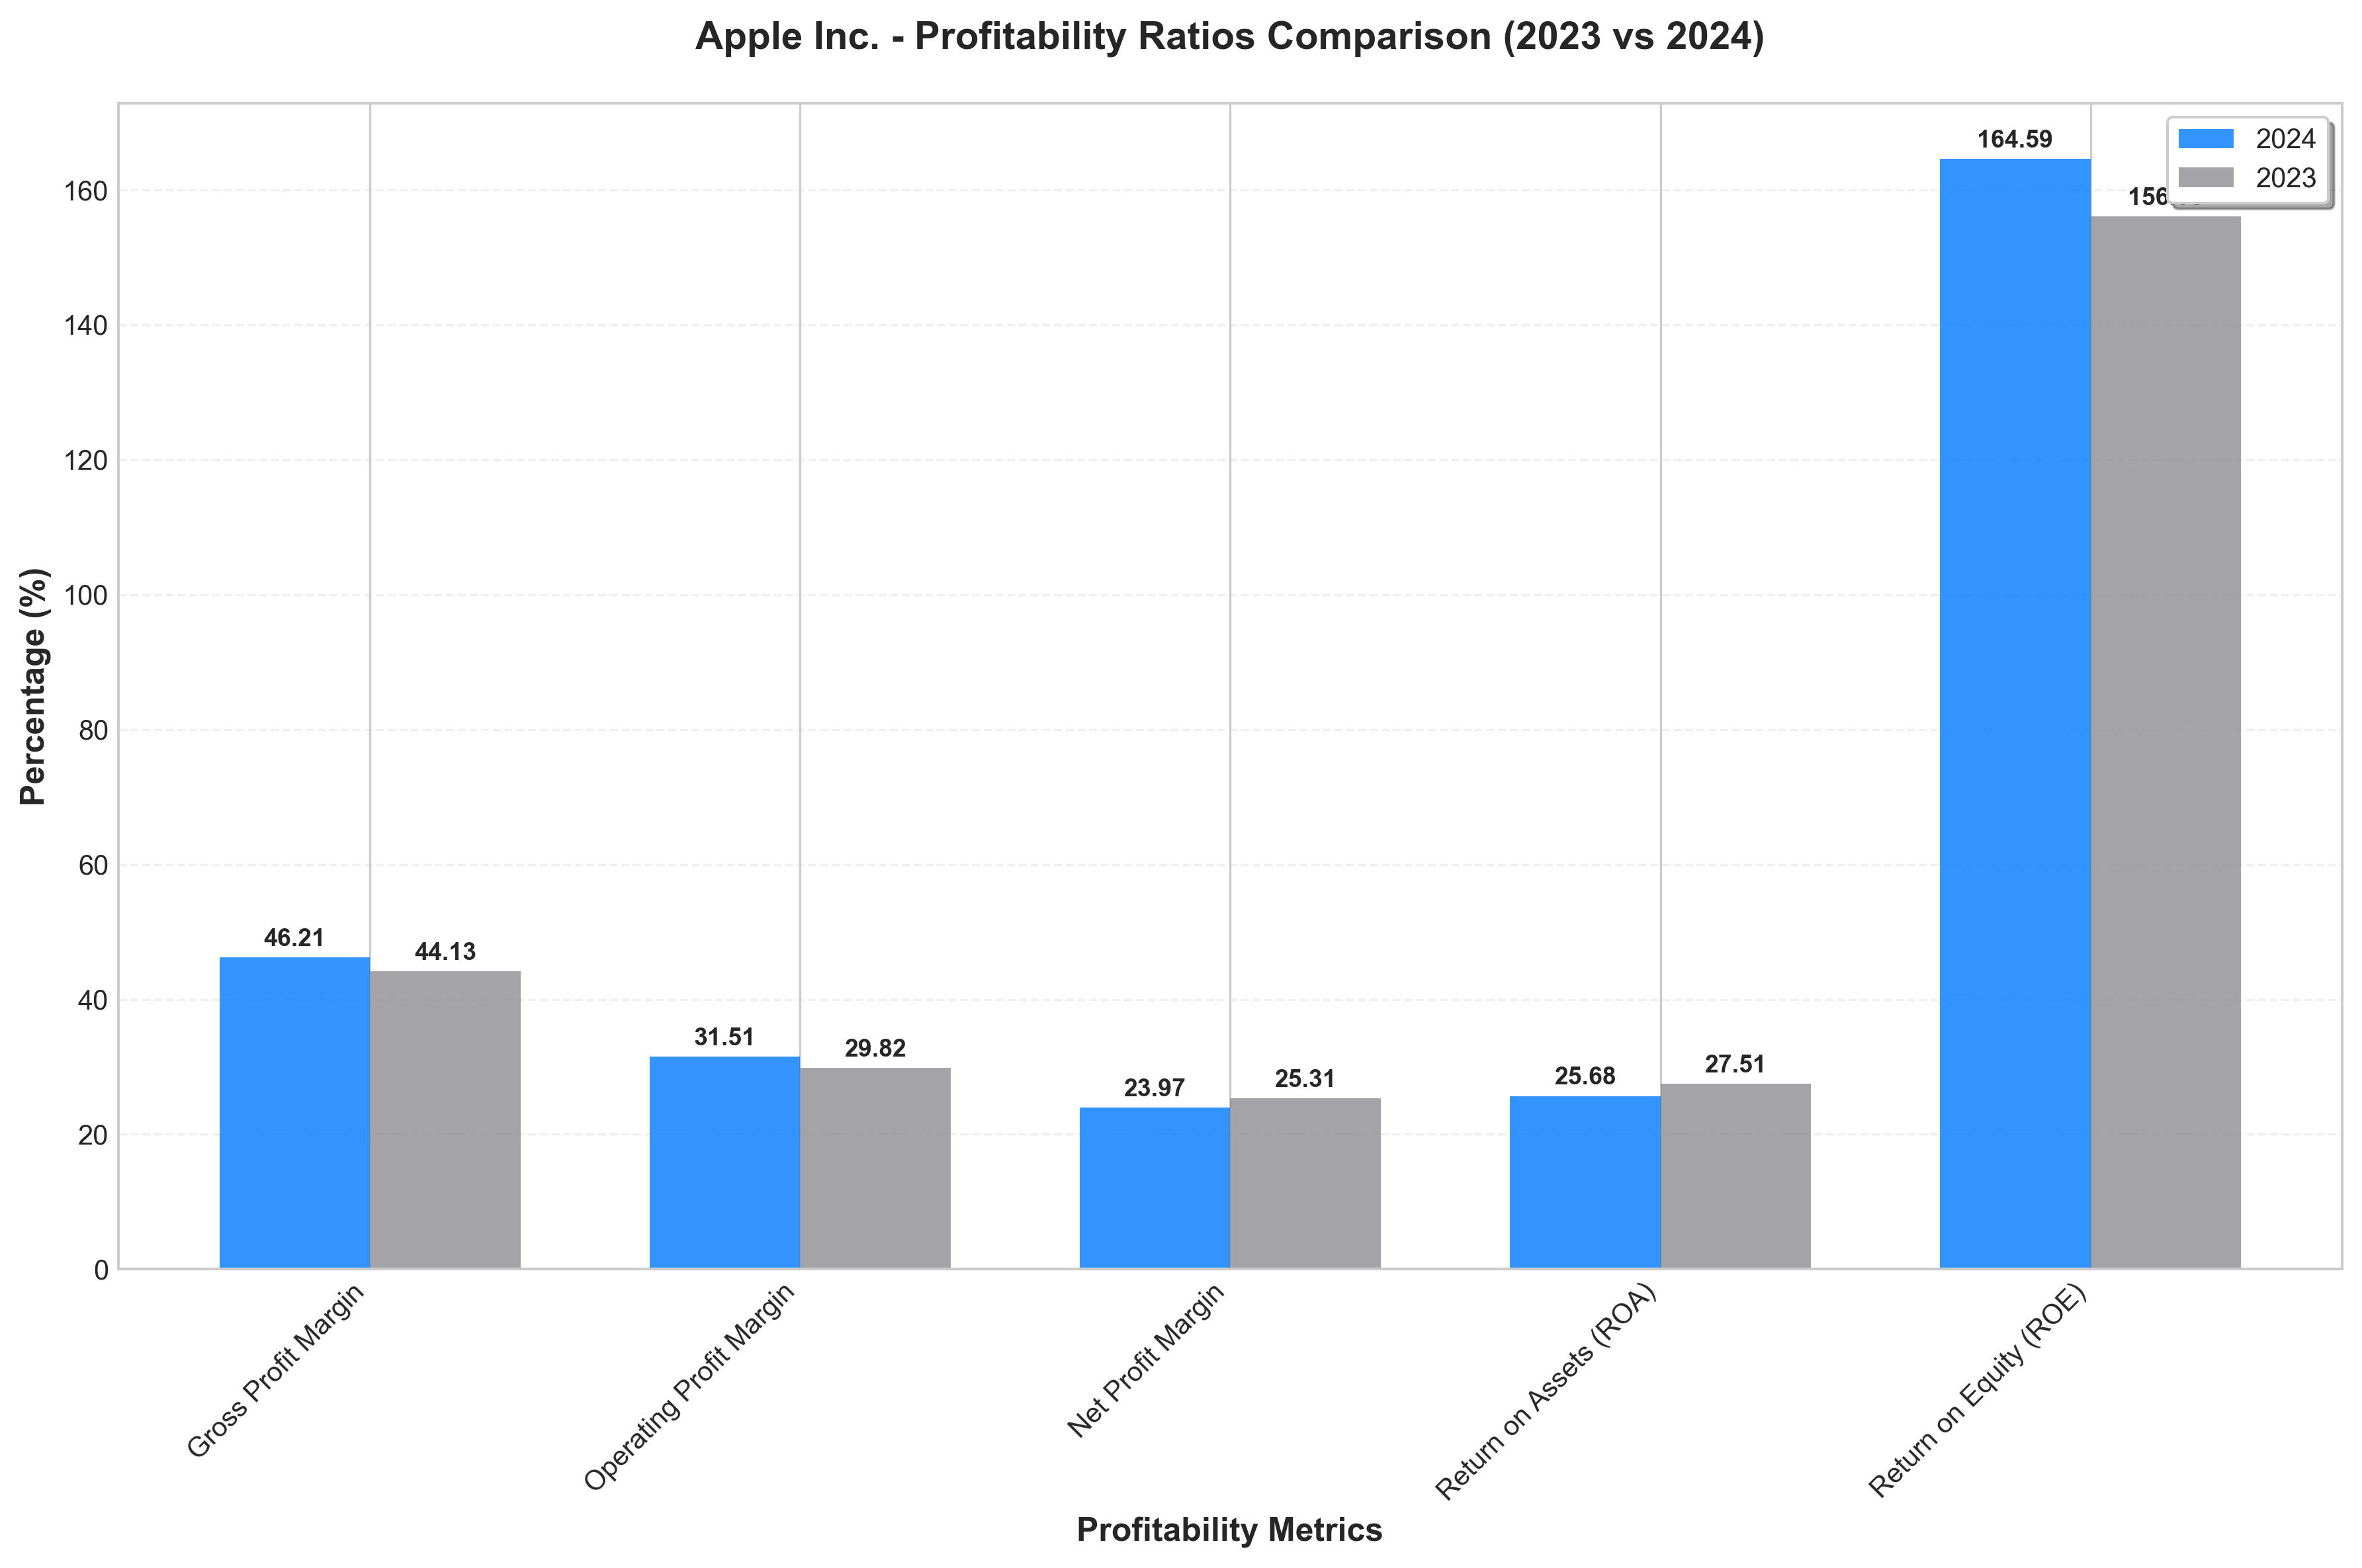
\includegraphics[width=0.9\textwidth]{figures/profitability_comparison.png}
\caption{Profitability Ratios Comparison (2023 vs 2024). Source: Computed from SEC Form 10-K data \citep{apple202410k}.}
\label{fig:profitability}
\end{figure}

\subsection{Liquidity Ratios}

Liquidity ratios measure the organisation's ability to meet short-term obligations using current assets. These ratios are critical for assessing working capital management and financial flexibility.

\subsubsection{Current Ratio}

The current ratio measures the organisation's ability to pay short-term obligations with current assets. This ratio was calculated as follows:

\begin{equation}
\mathrm{Current\ Ratio} = \frac{\mathrm{Total\ Current\ Assets}}{\mathrm{Total\ Current\ Liabilities}}
\end{equation}

\begin{table}[H]
\centering
\caption{Current Ratio Analysis (2023-2024)}
\label{tab:current_ratio}
\begin{tabular}{lrrr}
\toprule
\textbf{Year} & \textbf{Current Assets (\$M)} & \textbf{Current Liabilities (\$M)} & \textbf{Current Ratio} \\
\midrule
2024 & 152,987 & 176,392 & 0.87 \\
2023 & 143,566 & 145,308 & 0.99 \\
\textbf{Change} & +9,421 & +31,084 & \textbf{-0.12} \\
\bottomrule
\end{tabular}
\end{table}

As presented in Table~\ref{tab:current_ratio}, the current ratio fell from 0.99 in 2023 to 0.87 in 2024, dropping below the conventional 1.0 threshold. This decline reflects the organisation's strategic approach to working capital management rather than financial distress.

\paragraph{Interpretation}

A current ratio below 1.0 theoretically indicates that current liabilities exceed current assets, which would conventionally signal potential liquidity challenges. However, this ratio must be interpreted in context. Apple generates \$118.3 billion in operating cash flow annually, maintains \$65.2 billion in cash and marketable securities, and has access to substantial credit facilities. The decline of 0.12 represents a 12.2\% reduction from the prior year, the second-largest percentage decline among all ratios analysed \citep{apple202410k}.

The decline was driven primarily by a 21.4\% increase in current liabilities (from \$145.3 billion to \$176.4 billion) outpacing a 6.6\% increase in current assets (from \$143.6 billion to \$153.0 billion). The liability increase reflects higher accounts payable (\$6.3 billion increase) and commercial paper (\$4.0 billion increase) related to supply chain financing and working capital optimisation strategies \citep{apple202410k}.

The quick ratio measures the organisation's ability to meet short-term obligations with the most liquid assets. This ratio was calculated excluding inventories and prepaid expenses:

\begin{equation}
\mathrm{Quick\ Ratio} = \frac{\mathrm{Cash} + \mathrm{Marketable\ Securities} + \mathrm{Accounts\ Receivable}}{\mathrm{Total\ Current\ Liabilities}}
\end{equation}

\begin{table}[H]
\centering
\caption{Quick Ratio Analysis (2023-2024)}
\label{tab:quick_ratio}
\begin{tabular}{lrrr}
\toprule
\textbf{Year} & \textbf{Quick Assets (\$M)} & \textbf{Current Liabilities (\$M)} & \textbf{Quick Ratio} \\
\midrule
2024 & 98,581 & 176,392 & 0.56 \\
2023 & 91,063 & 145,308 & 0.63 \\
\textbf{Change} & +7,518 & +31,084 & \textbf{-0.07} \\
\bottomrule
\end{tabular}
\end{table}

\paragraph{Interpretation}

The quick ratio declined from 0.63 in 2023 to 0.56 in 2024, representing an 11.1\% reduction that signals reduced ability to meet immediate obligations without relying on inventory conversion. This ratio, excluding the \$7.3 billion in inventory that requires sales effort to convert to cash, provides the most conservative liquidity assessment \citep{apple202410k}.

Quick assets increased by \$7.5 billion (8.3\%) from 2023 to 2024, driven by higher cash and marketable securities, but this increase was overshadowed by the \$31.1 billion (21.4\%) increase in current liabilities. The quick ratio of 0.56 indicates that for every dollar of current liabilities, Apple has \$0.56 in immediately liquid assets. Whilst this ratio would concern most businesses, Apple's strong cash generation capacity and investment-grade credit rating mitigate immediate liquidity concerns \citep{kieso2023}.

\subsubsection{Cash Ratio}

The cash ratio measures the organisation's ability to meet short-term obligations with cash and marketable securities:

\begin{equation}
\mathrm{Cash\ Ratio} = \frac{\mathrm{Cash} + \mathrm{Marketable\ Securities}}{\mathrm{Total\ Current\ Liabilities}}
\end{equation}

\begin{table}[H]
\centering
\caption{Cash Ratio Analysis (2023-2024)}
\label{tab:cash_ratio}
\begin{tabular}{lrrr}
\toprule
\textbf{Year} & \textbf{Cash \& Securities (\$M)} & \textbf{Current Liabilities (\$M)} & \textbf{Cash Ratio} \\
\midrule
2024 & 65,171 & 176,392 & 0.37 \\
2023 & 61,555 & 145,308 & 0.42 \\
\textbf{Change} & +3,616 & +31,084 & \textbf{-0.05} \\
\bottomrule
\end{tabular}
\end{table}

\paragraph{Interpretation}

The cash ratio declined from 0.42 in 2023 to 0.37 in 2024, representing a 12.0\% reduction that marks the most significant liquidity deterioration. This ratio, considering only cash and marketable securities (totaling \$65.2 billion in 2024) without reliance on accounts receivable collection or inventory conversion, provides the most stringent test of immediate liquidity \citep{apple202410k}.

The cash ratio of 0.37 indicates that Apple's immediately available liquid assets cover only 37\% of current liabilities. However, this ratio must be interpreted in the context of Apple's business model, which generates substantial predictable cash flows from product sales and high-margin services subscriptions. The organisation's \$118.3 billion in annual operating cash flow exceeds total current liabilities of \$176.4 billion by 67\%, indicating strong ability to meet short-term obligations through ongoing operations \citep{kieso2023}.

Figure~\ref{fig:liquidity} presents a visual comparison of all three liquidity ratios for 2023 and 2024.

\begin{figure}[H]
\centering
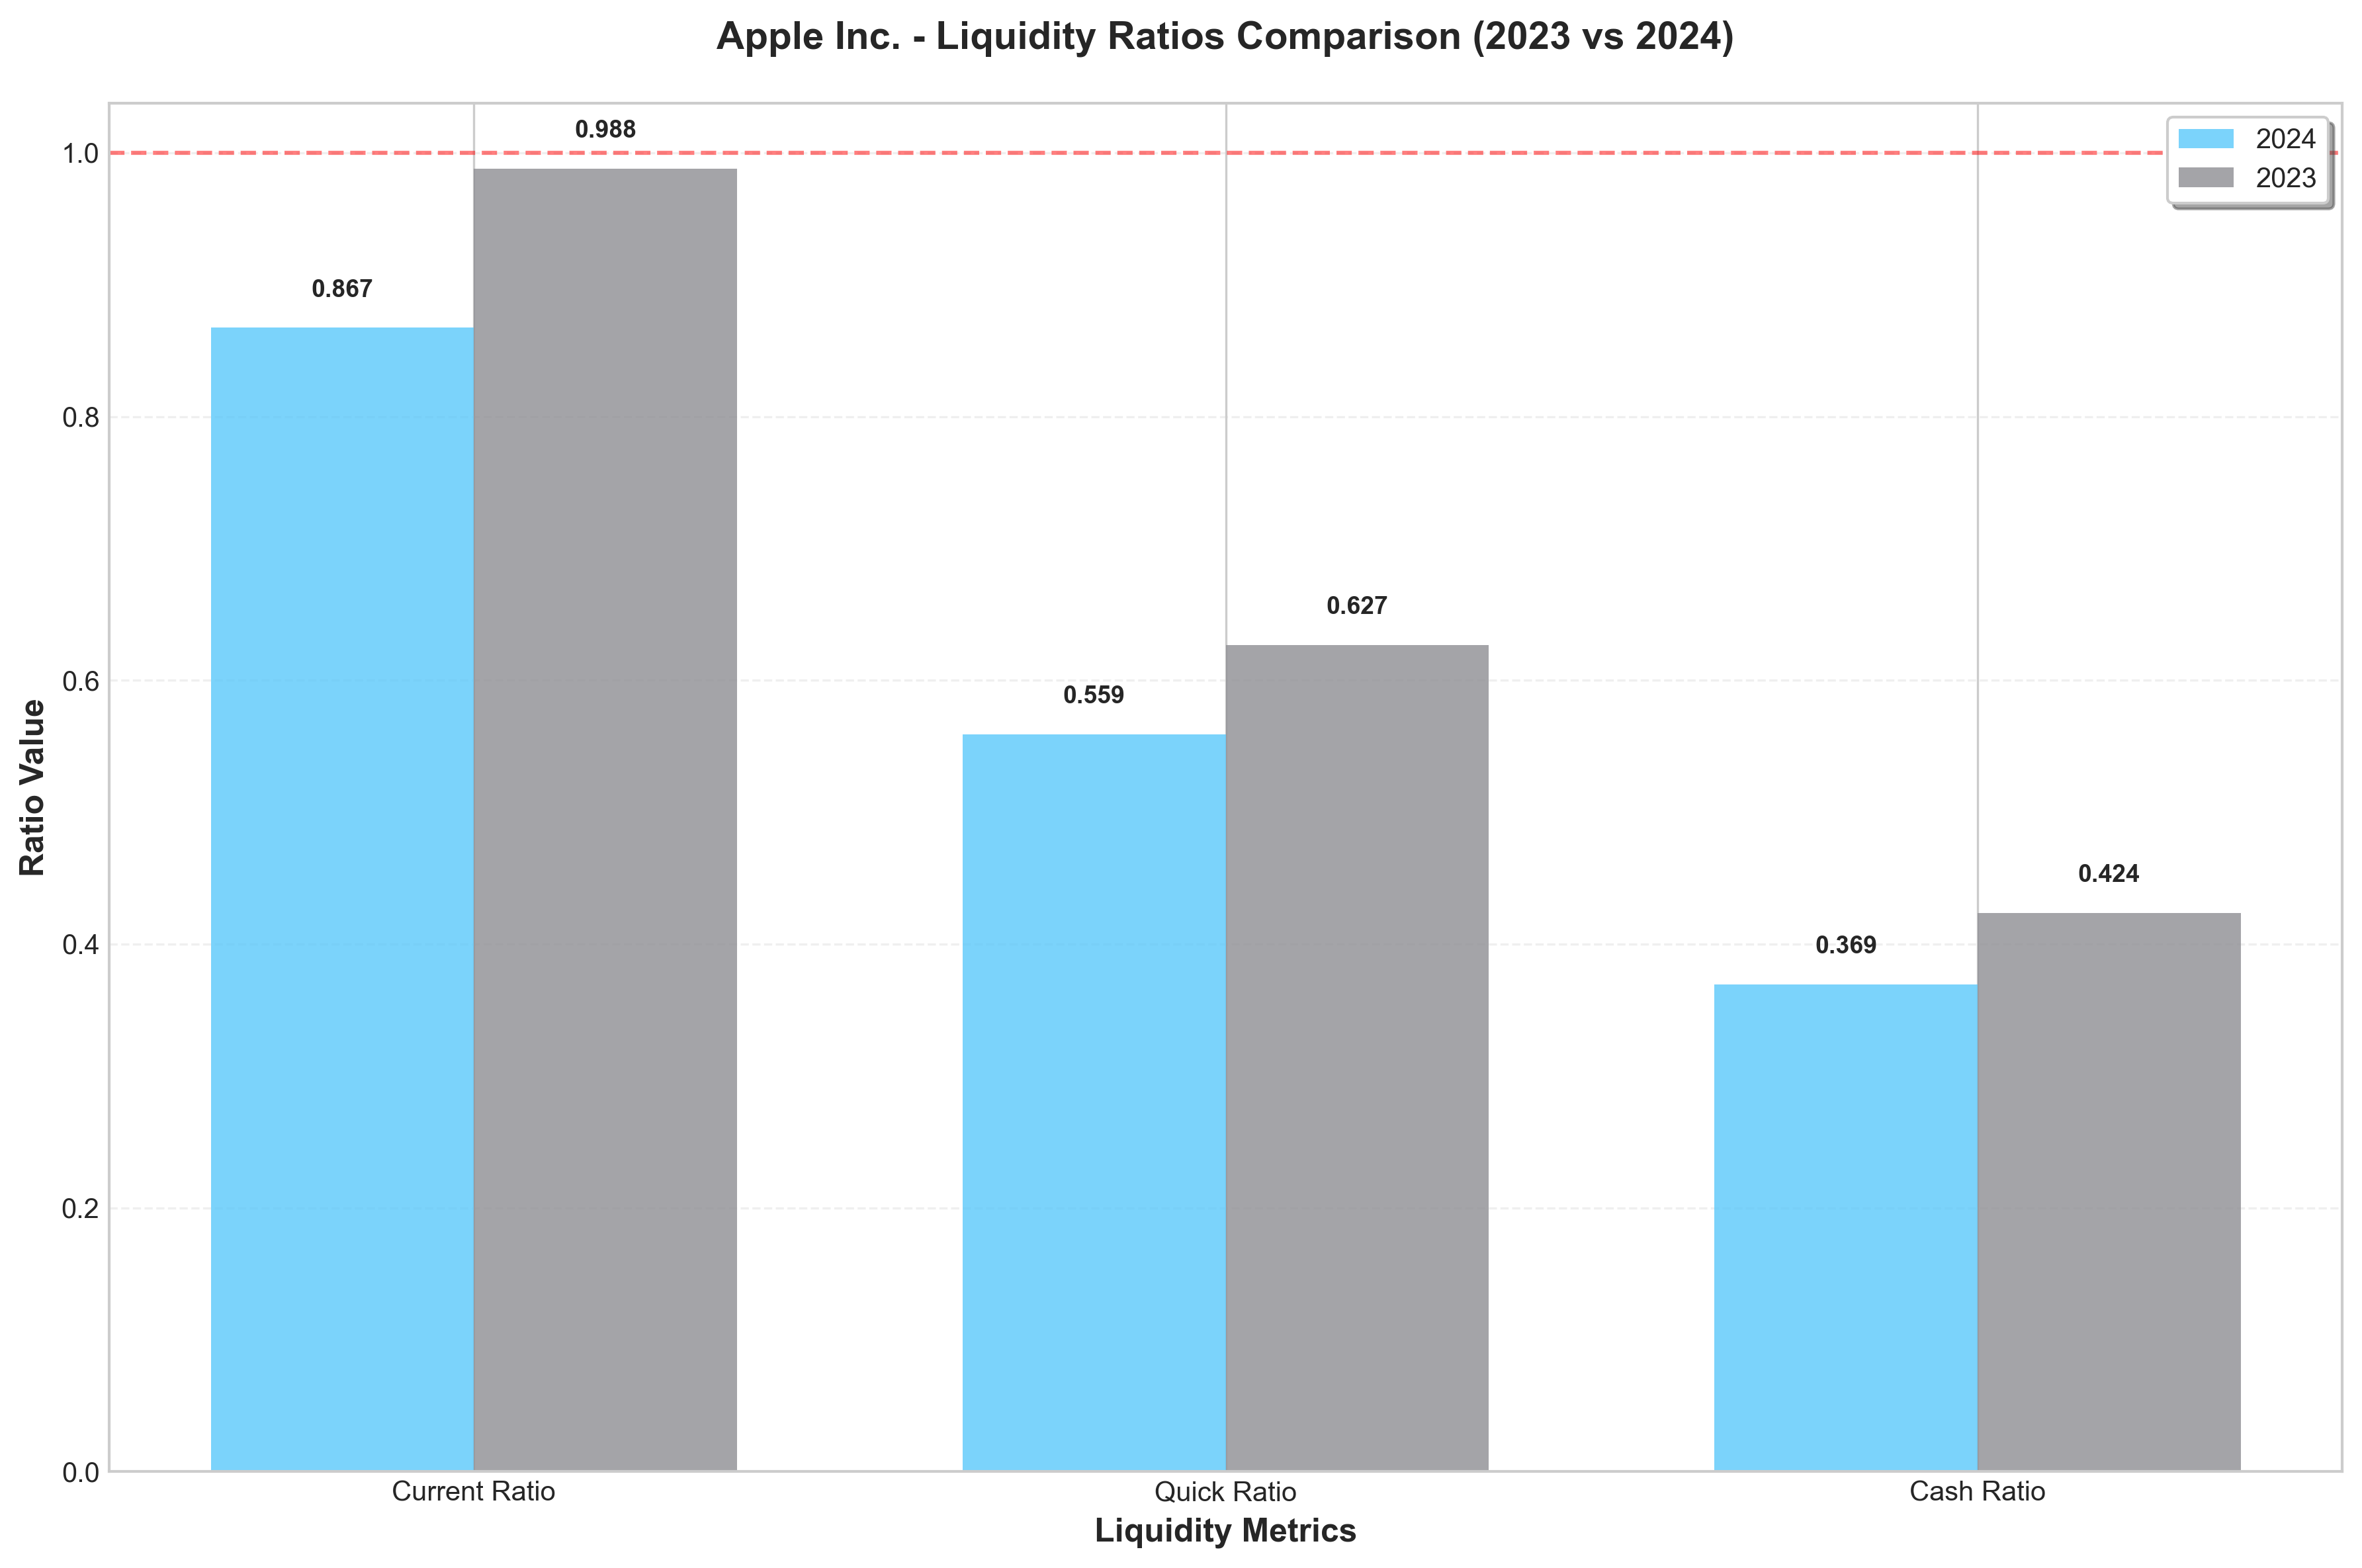
\includegraphics[width=0.9\textwidth]{figures/liquidity_ratios.png}
\caption{Liquidity Ratios Comparison (2023 vs 2024). Source: Computed from SEC Form 10-K data \citep{apple202410k}.}
\label{fig:liquidity}
\end{figure}

\subsection{Efficiency Ratios}

Efficiency ratios measure how effectively the organisation utilises its assets and manages its liabilities.

\subsubsection{Asset Turnover}

Asset turnover measures revenue generated per dollar of assets:

\begin{equation}
\mathrm{Asset\ Turnover} = \frac{\mathrm{Total\ Net\ Sales}}{\mathrm{Average\ Total\ Assets}}
\end{equation}

\begin{table}[H]
\centering
\caption{Asset Turnover Analysis (2023-2024)}
\label{tab:asset_turnover}
\begin{tabular}{lrrr}
\toprule
\textbf{Year} & \textbf{Net Sales (\$M)} & \textbf{Avg. Assets (\$M)} & \textbf{Asset Turnover (times)} \\
\midrule
2024 & 391,035 & 364,980 & 1.07 \\
2023 & 383,285 & 352,583 & 1.09 \\
\textbf{Change} & +7,750 & +12,397 & \textbf{-0.02} \\
\bottomrule
\end{tabular}
\end{table}

\paragraph{Interpretation}

Asset turnover declined from 1.09 times in 2023 to 1.07 times in 2024, indicating that each dollar of assets generated \$1.07 in revenue during 2024 compared to \$1.09 in the prior year. This 1.8\% decline reflects that asset growth (3.5\% increase) outpaced revenue growth (2.0\% increase) \citep{apple202410k}.

The asset turnover ratio measures how efficiently the organisation utilises its asset base to generate sales. Apple's ratio of 1.07 indicates that \$1 of assets generates approximately \$1.07 in annual revenue. This ratio is significantly lower than some technology peers due to Apple's substantial cash and marketable securities holdings (\$227 billion), which inflate the asset base without directly contributing to revenue generation. Excluding cash and marketable securities, the adjusted asset turnover would be substantially higher \citep{kieso2023}.

\subsubsection{Inventory Turnover}

Inventory turnover measures how efficiently inventory is managed:

\begin{equation}
\mathrm{Inventory\ Turnover} = \frac{\mathrm{Cost\ of\ Sales}}{\mathrm{Average\ Inventory}}
\end{equation}

\begin{table}[H]
\centering
\caption{Inventory Turnover Analysis (2023-2024)}
\label{tab:inventory_turnover}
\begin{tabular}{lrrr}
\toprule
\textbf{Year} & \textbf{Cost of Sales (\$M)} & \textbf{Avg. Inventory (\$M)} & \textbf{Inventory Turnover (times)} \\
\midrule
2024 & 210,352 & 6,809 & 53.67 \\
2023 & 214,137 & 6,331 & 60.54 \\
\textbf{Change} & -3,785 & +478 & \textbf{-6.87} \\
\bottomrule
\end{tabular}
\end{table}

\paragraph{Interpretation}

Inventory turnover declined from 60.54 times in 2023 to 53.67 times in 2024, representing an 11.3\% deterioration. This ratio indicates that inventory was sold and replenished approximately 53.7 times during 2024, equivalent to turning over the entire inventory approximately every 6.8 days \citep{apple202410k}.

Despite the decline, this ratio remains exceptionally high compared to technology industry averages of approximately 7-10 times annually. The exceptional turnover reflects Apple's world-class supply chain management, just-in-time inventory practices, and strong product demand that minimises inventory holding periods. The decline from 2023 may reflect changes in product mix, introduction of new product lines requiring component accumulation, or strategic inventory buildup ahead of product launches \citep{unleashed2024}.

\subsubsection{Days Inventory Outstanding}

Days inventory outstanding indicates the average number of days inventory is held:

\begin{equation}
\mathrm{Days\ Inventory\ Outstanding} = \frac{365}{\mathrm{Inventory\ Turnover}}
\end{equation}

\begin{table}[H]
\centering
\caption{Days Inventory Outstanding Analysis (2023-2024)}
\label{tab:dio}
\begin{tabular}{lrr}
\toprule
\textbf{Year} & \textbf{Days Inventory Outstanding (days)} \\
\midrule
2024 & 6.80 \\
2023 & 6.03 \\
\textbf{Change} & +0.77 \\
\bottomrule
\end{tabular}
\end{table}

\paragraph{Interpretation}

Days inventory outstanding increased from 6.03 days in 2023 to 6.80 days in 2024, representing a 12.8\% increase. This metric indicates that the average inventory item was held for approximately 6.8 days before being sold, compared to 6.0 days in the prior year \citep{apple202410k}.

This increase, while modest, corroborates the decline in inventory turnover and suggests a slight lengthening of the inventory conversion cycle. However, the DIO of 6.8 days remains extraordinarily low relative to technology industry averages of 30-60 days, reinforcing Apple's supply chain excellence. The minimal inventory holding period reduces carrying costs, obsolescence risk, and working capital tied up in inventory \citep{kieso2023}.

\subsubsection{Accounts Receivable Turnover}

Accounts receivable turnover measures how efficiently credit sales are collected:

\begin{equation}
\mathrm{Accounts\ Receivable\ Turnover} = \frac{\mathrm{Total\ Net\ Sales}}{\mathrm{Average\ Accounts\ Receivable}}
\end{equation}

\begin{table}[H]
\centering
\caption{Accounts Receivable Turnover Analysis (2023-2024)}
\label{tab:ar_turnover}
\begin{tabular}{lrrr}
\toprule
\textbf{Year} & \textbf{Net Sales (\$M)} & \textbf{Avg. AR (\$M)} & \textbf{AR Turnover (times)} \\
\midrule
2024 & 391,035 & 31,459 & 11.70 \\
2023 & 383,285 & 30,008 & 12.99 \\
\textbf{Change} & +7,750 & +1,451 & \textbf{-1.29} \\
\bottomrule
\end{tabular}
\end{table}

\paragraph{Interpretation}

Accounts receivable turnover declined from 12.99 times in 2023 to 11.70 times in 2024, representing a 9.9\% reduction. This ratio indicates that accounts receivable were collected approximately 11.7 times during 2024, meaning the average receivable was outstanding for approximately 31 days before collection \citep{apple202410k}.

The decline reflects the increase in average accounts receivable from \$30.0 billion to \$31.5 billion (up 5.0\%) outpacing revenue growth of 2.0\%. This may indicate longer payment terms offered to distributors and carriers, or slower collection from enterprise customers. However, the turnover of 11.7 times remains strong, indicating effective credit management and collection processes \citep{kieso2023}.

\subsubsection{Days Sales Outstanding}

Days sales outstanding indicates the average collection period:

\begin{equation}
\mathrm{Days\ Sales\ Outstanding} = \frac{365}{\mathrm{Accounts\ Receivable\ Turnover}}
\end{equation}

\begin{table}[H]
\centering
\caption{Days Sales Outstanding Analysis (2023-2024)}
\label{tab:dso}
\begin{tabular}{lrr}
\toprule
\textbf{Year} & \textbf{Days Sales Outstanding (days)} \\
\midrule
2024 & 31.19 \\
2023 & 28.10 \\
\textbf{Change} & +3.09 \\
\bottomrule
\end{tabular}
\end{table}

\paragraph{Interpretation}

Days sales outstanding increased from 28.10 days in 2023 to 31.19 days in 2024, representing an 11.0\% extension of the average collection period. This metric indicates that the average receivable remained outstanding for 31.2 days before being collected, compared to 28.1 days in the prior year \citep{apple202410k}.

The increase of 3.09 days in the collection period represents a meaningful deterioration in receivables management efficiency. This extension of credit terms, whether intentional or due to collection challenges, impacts working capital by delaying cash conversion. The DSO of 31.2 days, combined with the DIO of 6.8 days, yields a cash conversion cycle of approximately 38 days, meaning nearly five weeks elapse between cash outflow for inventory and cash inflow from sales \citep{kieso2023}.

Figure~\ref{fig:efficiency} presents a visual comparison of all five efficiency ratios for 2023 and 2024.

\begin{figure}[H]
\centering
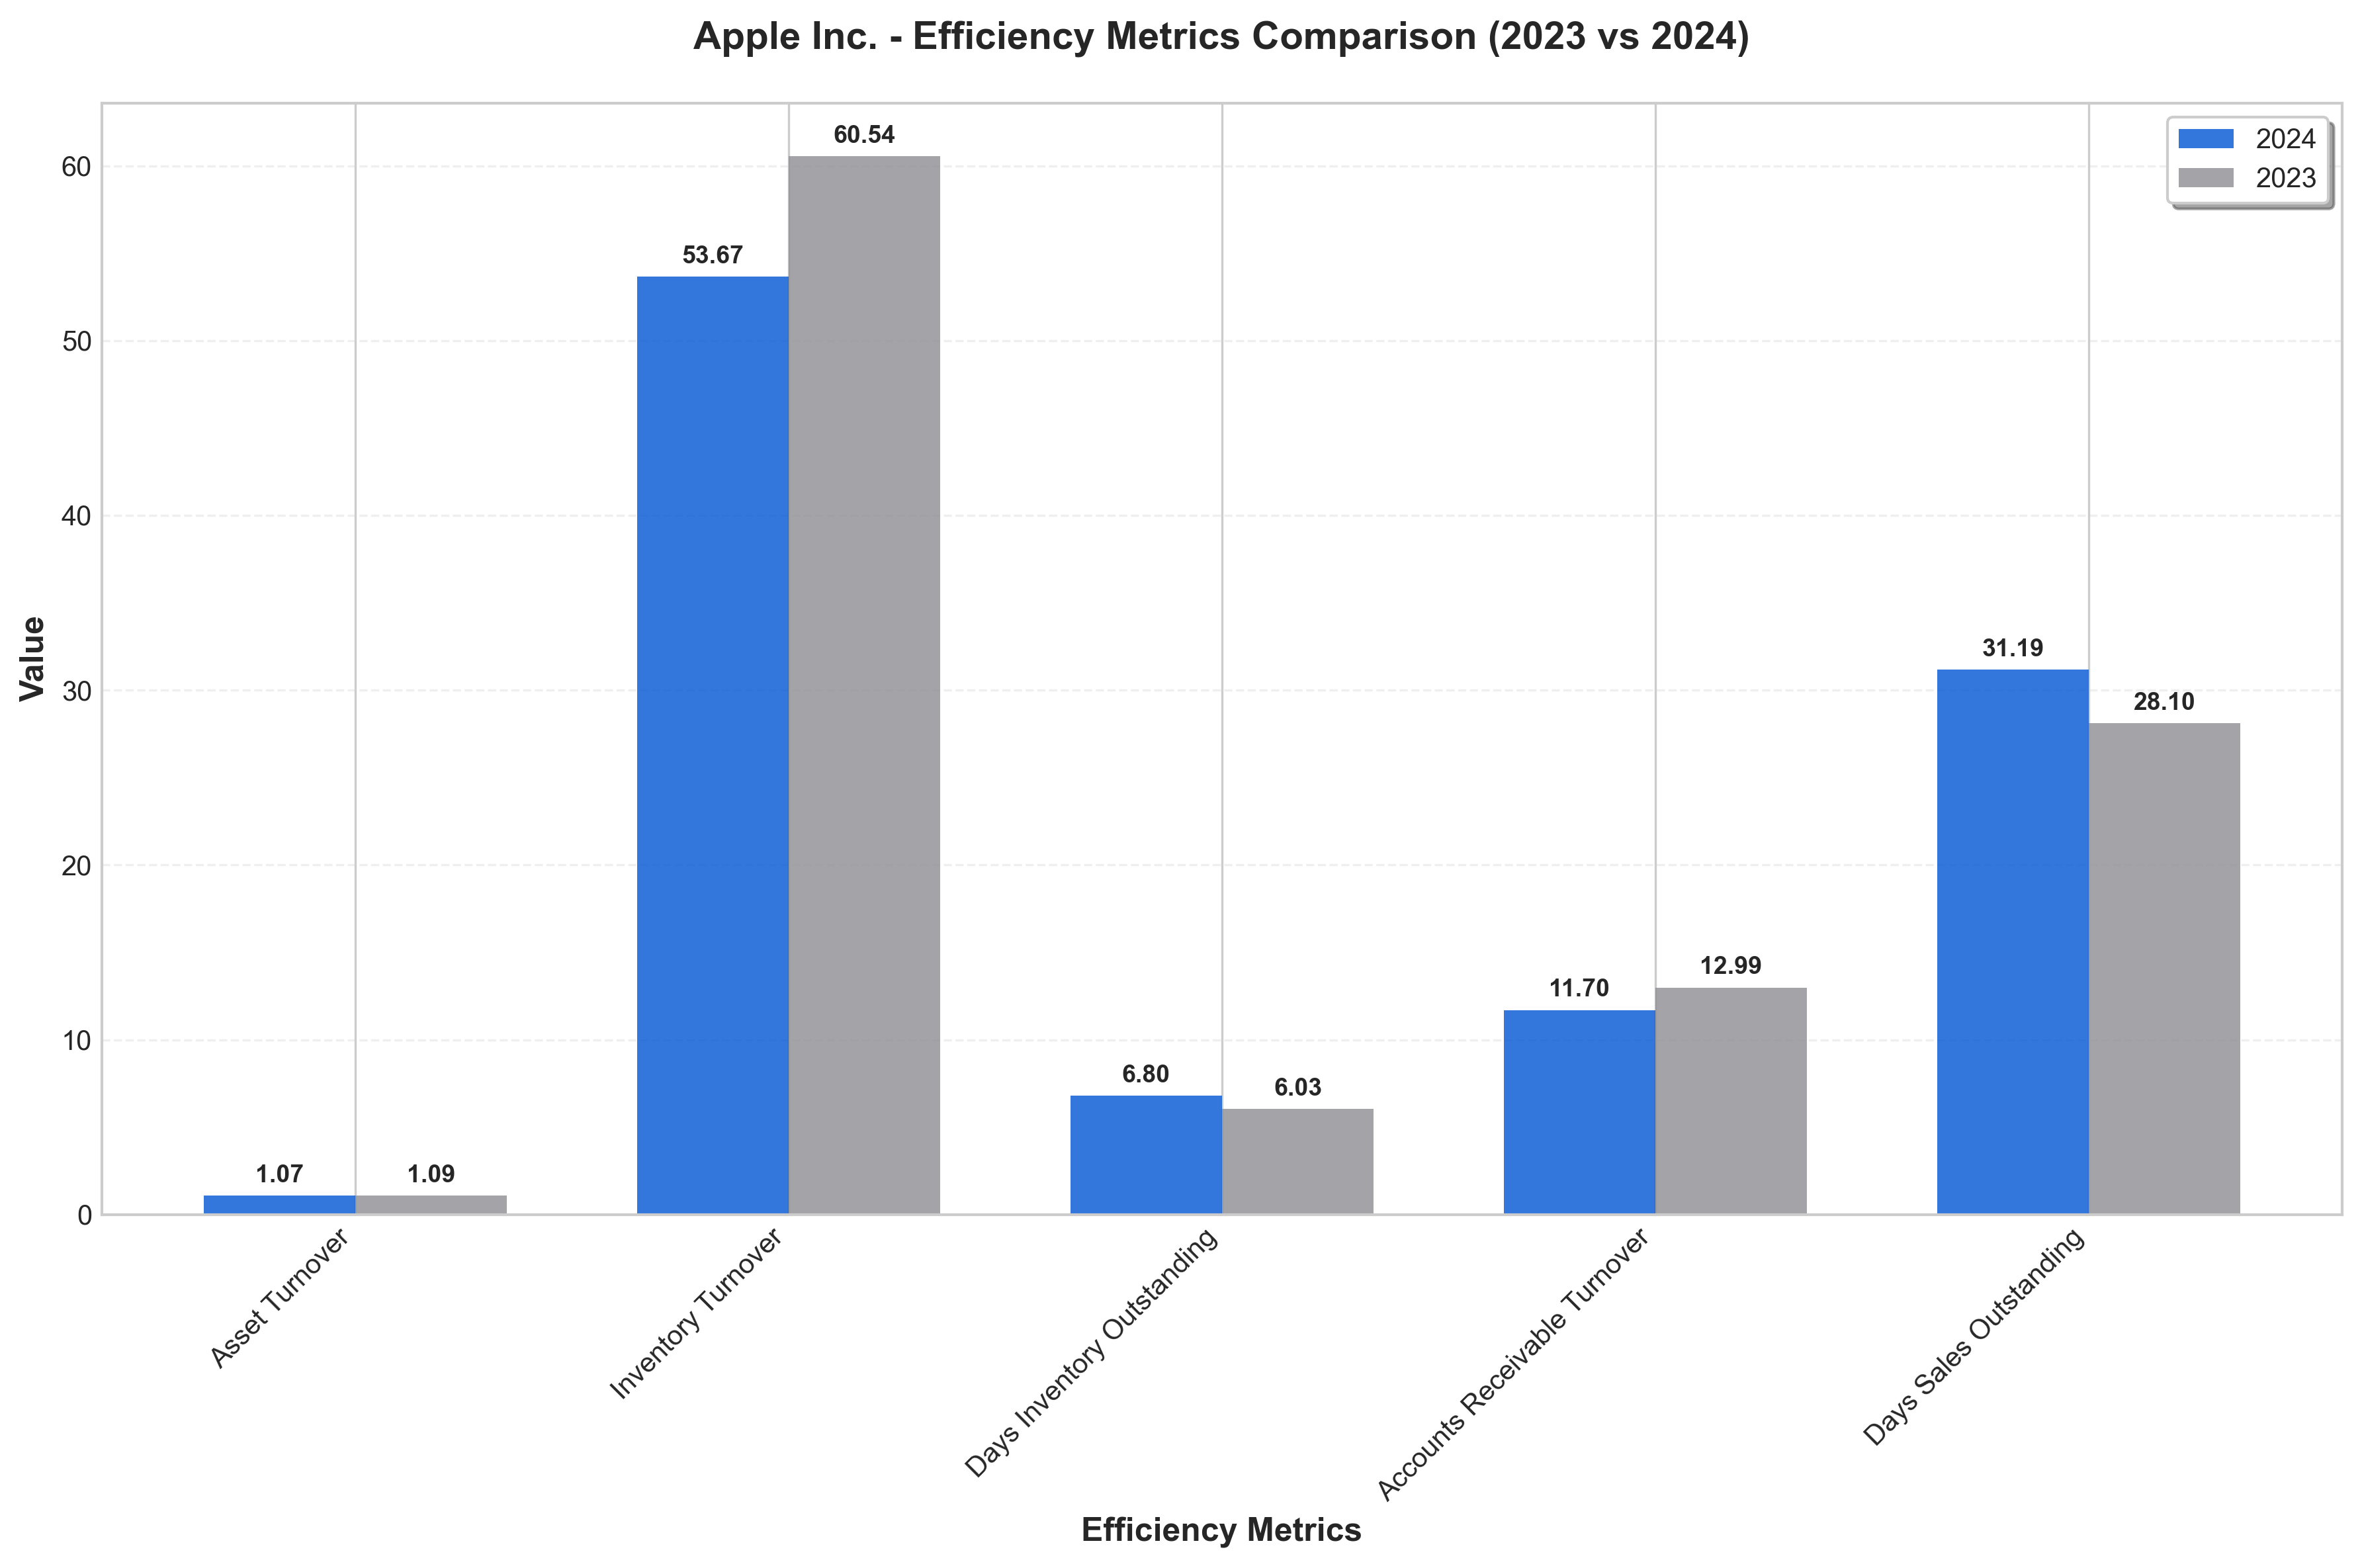
\includegraphics[width=0.9\textwidth]{figures/efficiency_metrics.png}
\caption{Efficiency Metrics Comparison (2023 vs 2024). Source: Computed from SEC Form 10-K data \citep{apple202410k}.}
\label{fig:efficiency}
\end{figure}

\subsection{Gearing Ratios}

Gearing ratios measure the organisation's financial leverage and capital structure.

\subsubsection{Debt to Equity Ratio}

The debt to equity ratio measures financial leverage:

\begin{equation}
\mathrm{Debt\ to\ Equity} = \frac{\mathrm{Total\ Debt}}{\mathrm{Total\ Shareholders'\ Equity}}
\end{equation}

\begin{table}[H]
\centering
\caption{Debt to Equity Ratio Analysis (2023-2024)}
\label{tab:de}
\begin{tabular}{lrrr}
\toprule
\textbf{Year} & \textbf{Total Debt (\$M)} & \textbf{Equity (\$M)} & \textbf{Debt to Equity} \\
\midrule
2024 & 96,662 & 56,950 & 1.70 \\
2023 & 105,103 & 62,146 & 1.69 \\
\textbf{Change} & -8,441 & -5,196 & \textbf{+0.01} \\
\bottomrule
\end{tabular}
\end{table}

\paragraph{Interpretation}

The debt to equity ratio increased from 1.69 in 2023 to 1.70 in 2024, remaining essentially stable. This ratio indicates that for every dollar of shareholders' equity, Apple employs \$1.70 of debt, representing high financial leverage. The ratio is 143\% higher than the technology industry benchmark of 0.7, indicating significantly greater use of debt financing than typical technology companies \citep{readyratios2024}.

The stable leverage position reflects deliberate capital structure management. Total debt decreased by \$8.4 billion (8.0\%) whilst shareholders' equity decreased by \$5.2 billion (8.4\%), largely due to aggressive share repurchases that reduce equity. The high leverage amplifies returns to equity holders (evidenced by the extraordinary ROE of 164.59\%) but also increases financial risk. However, Apple's strong cash generation and investment-grade credit rating mitigate default risk \citep{brealey2020}.

\subsubsection{Debt to Assets Ratio}

The debt to assets ratio measures the proportion of assets financed through debt:

\begin{equation}
\mathrm{Debt\ to\ Assets} = \frac{\mathrm{Total\ Debt}}{\mathrm{Total\ Assets}}
\end{equation}

\begin{table}[H]
\centering
\caption{Debt to Assets Ratio Analysis (2023-2024)}
\label{tab:da}
\begin{tabular}{lrrr}
\toprule
\textbf{Year} & \textbf{Total Debt (\$M)} & \textbf{Assets (\$M)} & \textbf{Debt to Assets} \\
\midrule
2024 & 96,662 & 364,980 & 0.26 \\
2023 & 105,103 & 352,583 & 0.30 \\
\textbf{Change} & -8,441 & +12,397 & \textbf{-0.03} \\
\bottomrule
\end{tabular}
\end{table}

\paragraph{Interpretation}

The debt to assets ratio improved from 0.30 in 2023 to 0.26 in 2024, indicating that 26\% of total assets were financed through debt in 2024 compared to 30\% in 2023. This 10.0\% reduction reflects the decrease in total debt coupled with asset base expansion. The ratio indicates that Apple maintains a conservative approach to debt financing relative to total assets, with the majority of assets (74\%) financed through equity and liabilities other than interest-bearing debt \citep{apple202410k}.

The improvement in this ratio strengthens the balance sheet and reduces financial risk. The organisation's debt portfolio consists primarily of fixed-rate notes with interest rates ranging from 0.5\% to 4.7\% and maturities extending through 2052, providing predictability of debt service costs. The reduction in leverage enhances financial flexibility for future strategic initiatives \citep{kieso2023}.

\subsubsection{Equity Ratio}

The equity ratio measures the proportion of assets financed through equity:

\begin{equation}
\mathrm{Equity\ Ratio} = \frac{\mathrm{Total\ Shareholders'\ Equity}}{\mathrm{Total\ Assets}}
\end{equation}

\begin{table}[H]
\centering
\caption{Equity Ratio Analysis (2023-2024)}
\label{tab:equity_ratio}
\begin{tabular}{lrrr}
\toprule
\textbf{Year} & \textbf{Equity (\$M)} & \textbf{Assets (\$M)} & \textbf{Equity Ratio} \\
\midrule
2024 & 56,950 & 364,980 & 0.16 \\
2023 & 62,146 & 352,583 & 0.18 \\
\textbf{Change} & -5,196 & +12,397 & \textbf{-0.02} \\
\bottomrule
\end{tabular}
\end{table}

\paragraph{Interpretation}

The equity ratio declined from 0.18 in 2023 to 0.16 in 2024, indicating that 16\% of total assets were financed through shareholders' equity in 2024 compared to 18\% in 2023. This 11.1\% reduction reflects the decrease in shareholders' equity from \$62.1 billion to \$57.0 billion, primarily driven by share repurchases and dividends that exceeded net income for the period \citep{apple202410k}.

The declining equity ratio is a direct consequence of Apple's capital return strategy. By repurchasing \$95.0 billion of shares in 2024, the organisation reduces shareholders' equity whilst maintaining or increasing earnings, thereby boosting return on equity. The low equity ratio of 0.16 indicates high financial leverage but must be evaluated in the context of Apple's strong cash generation and debt service capacity \citep{brealey2020}.

Figure~\ref{fig:gearing} presents a visual comparison of all three gearing ratios for 2023 and 2024.

\begin{figure}[H]
\centering
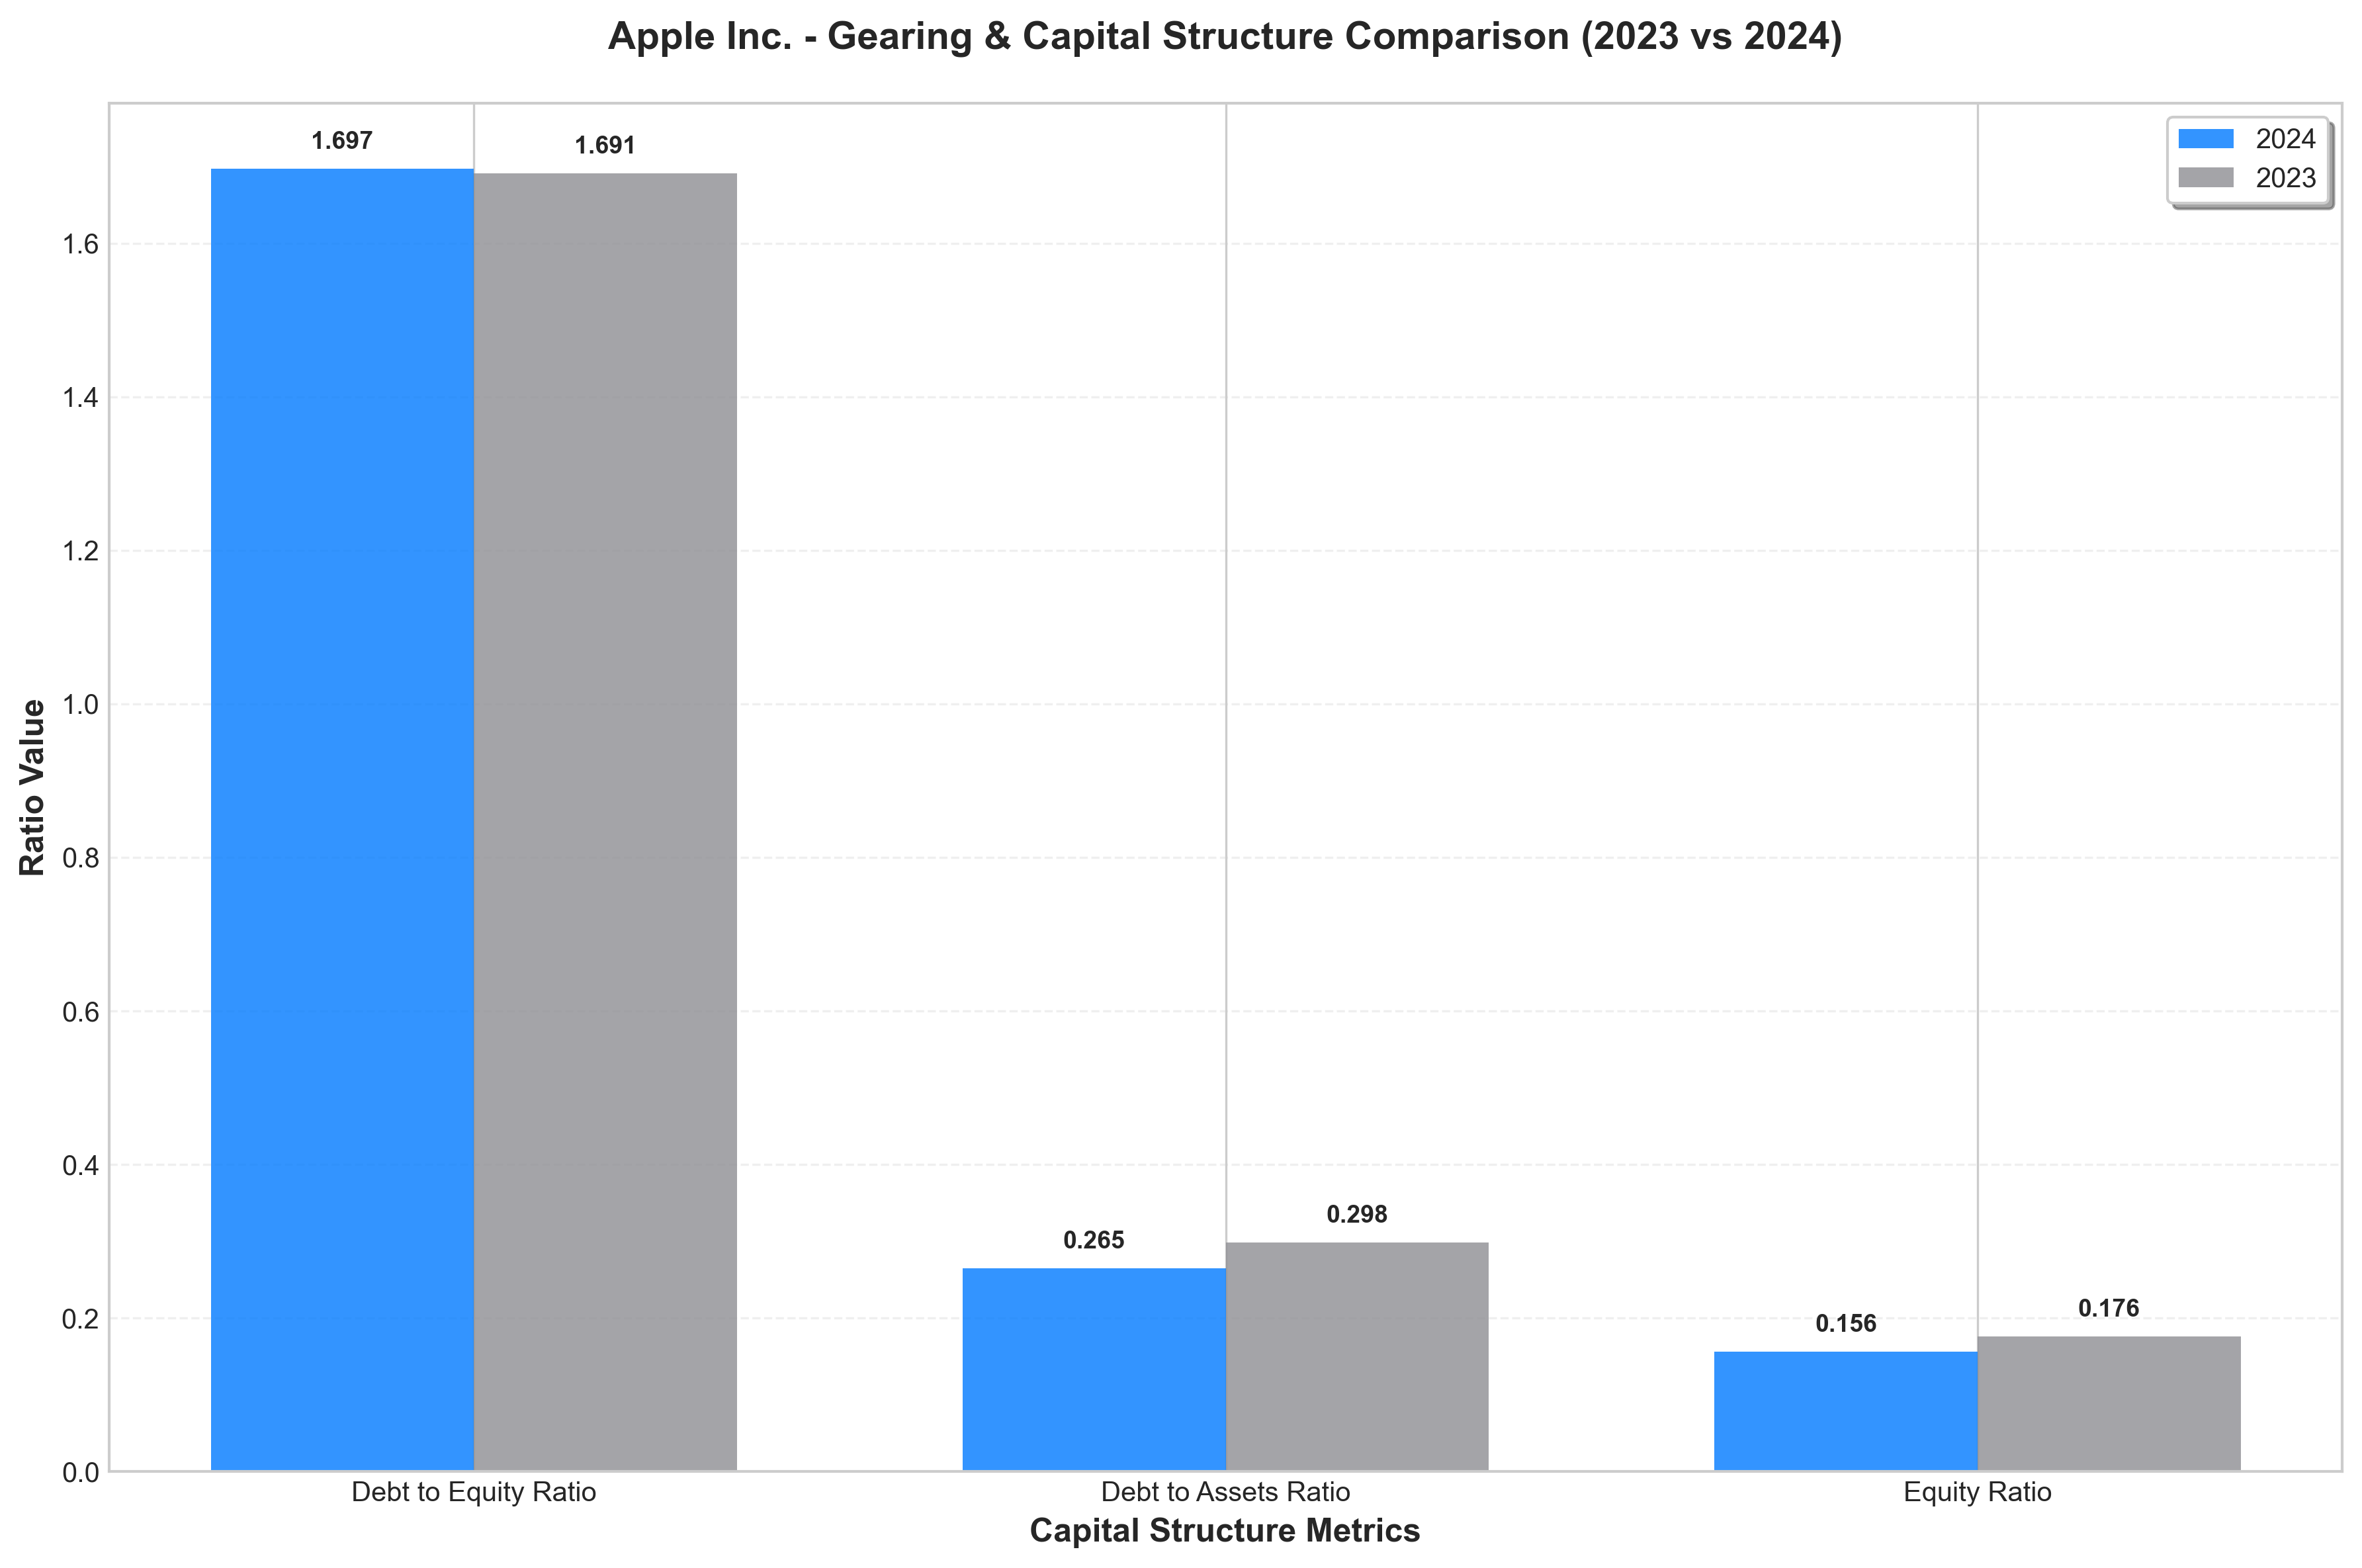
\includegraphics[width=0.9\textwidth]{figures/gearing_ratios.png}
\caption{Gearing Ratios Comparison (2023 vs 2024). Source: Computed from SEC Form 10-K data \citep{apple202410k}.}
\label{fig:gearing}
\end{figure}

\subsection{Extended Financial Analysis}

\subsubsection{Year-over-Year Change Analysis}

Figure~\ref{fig:yoy_change} presents a comprehensive analysis of year-over-year changes across all 17 financial ratios. The analysis indicated that six ratios showed improvement whilst eleven ratios showed decline from 2023 to 2024.

\begin{figure}[H]
\centering
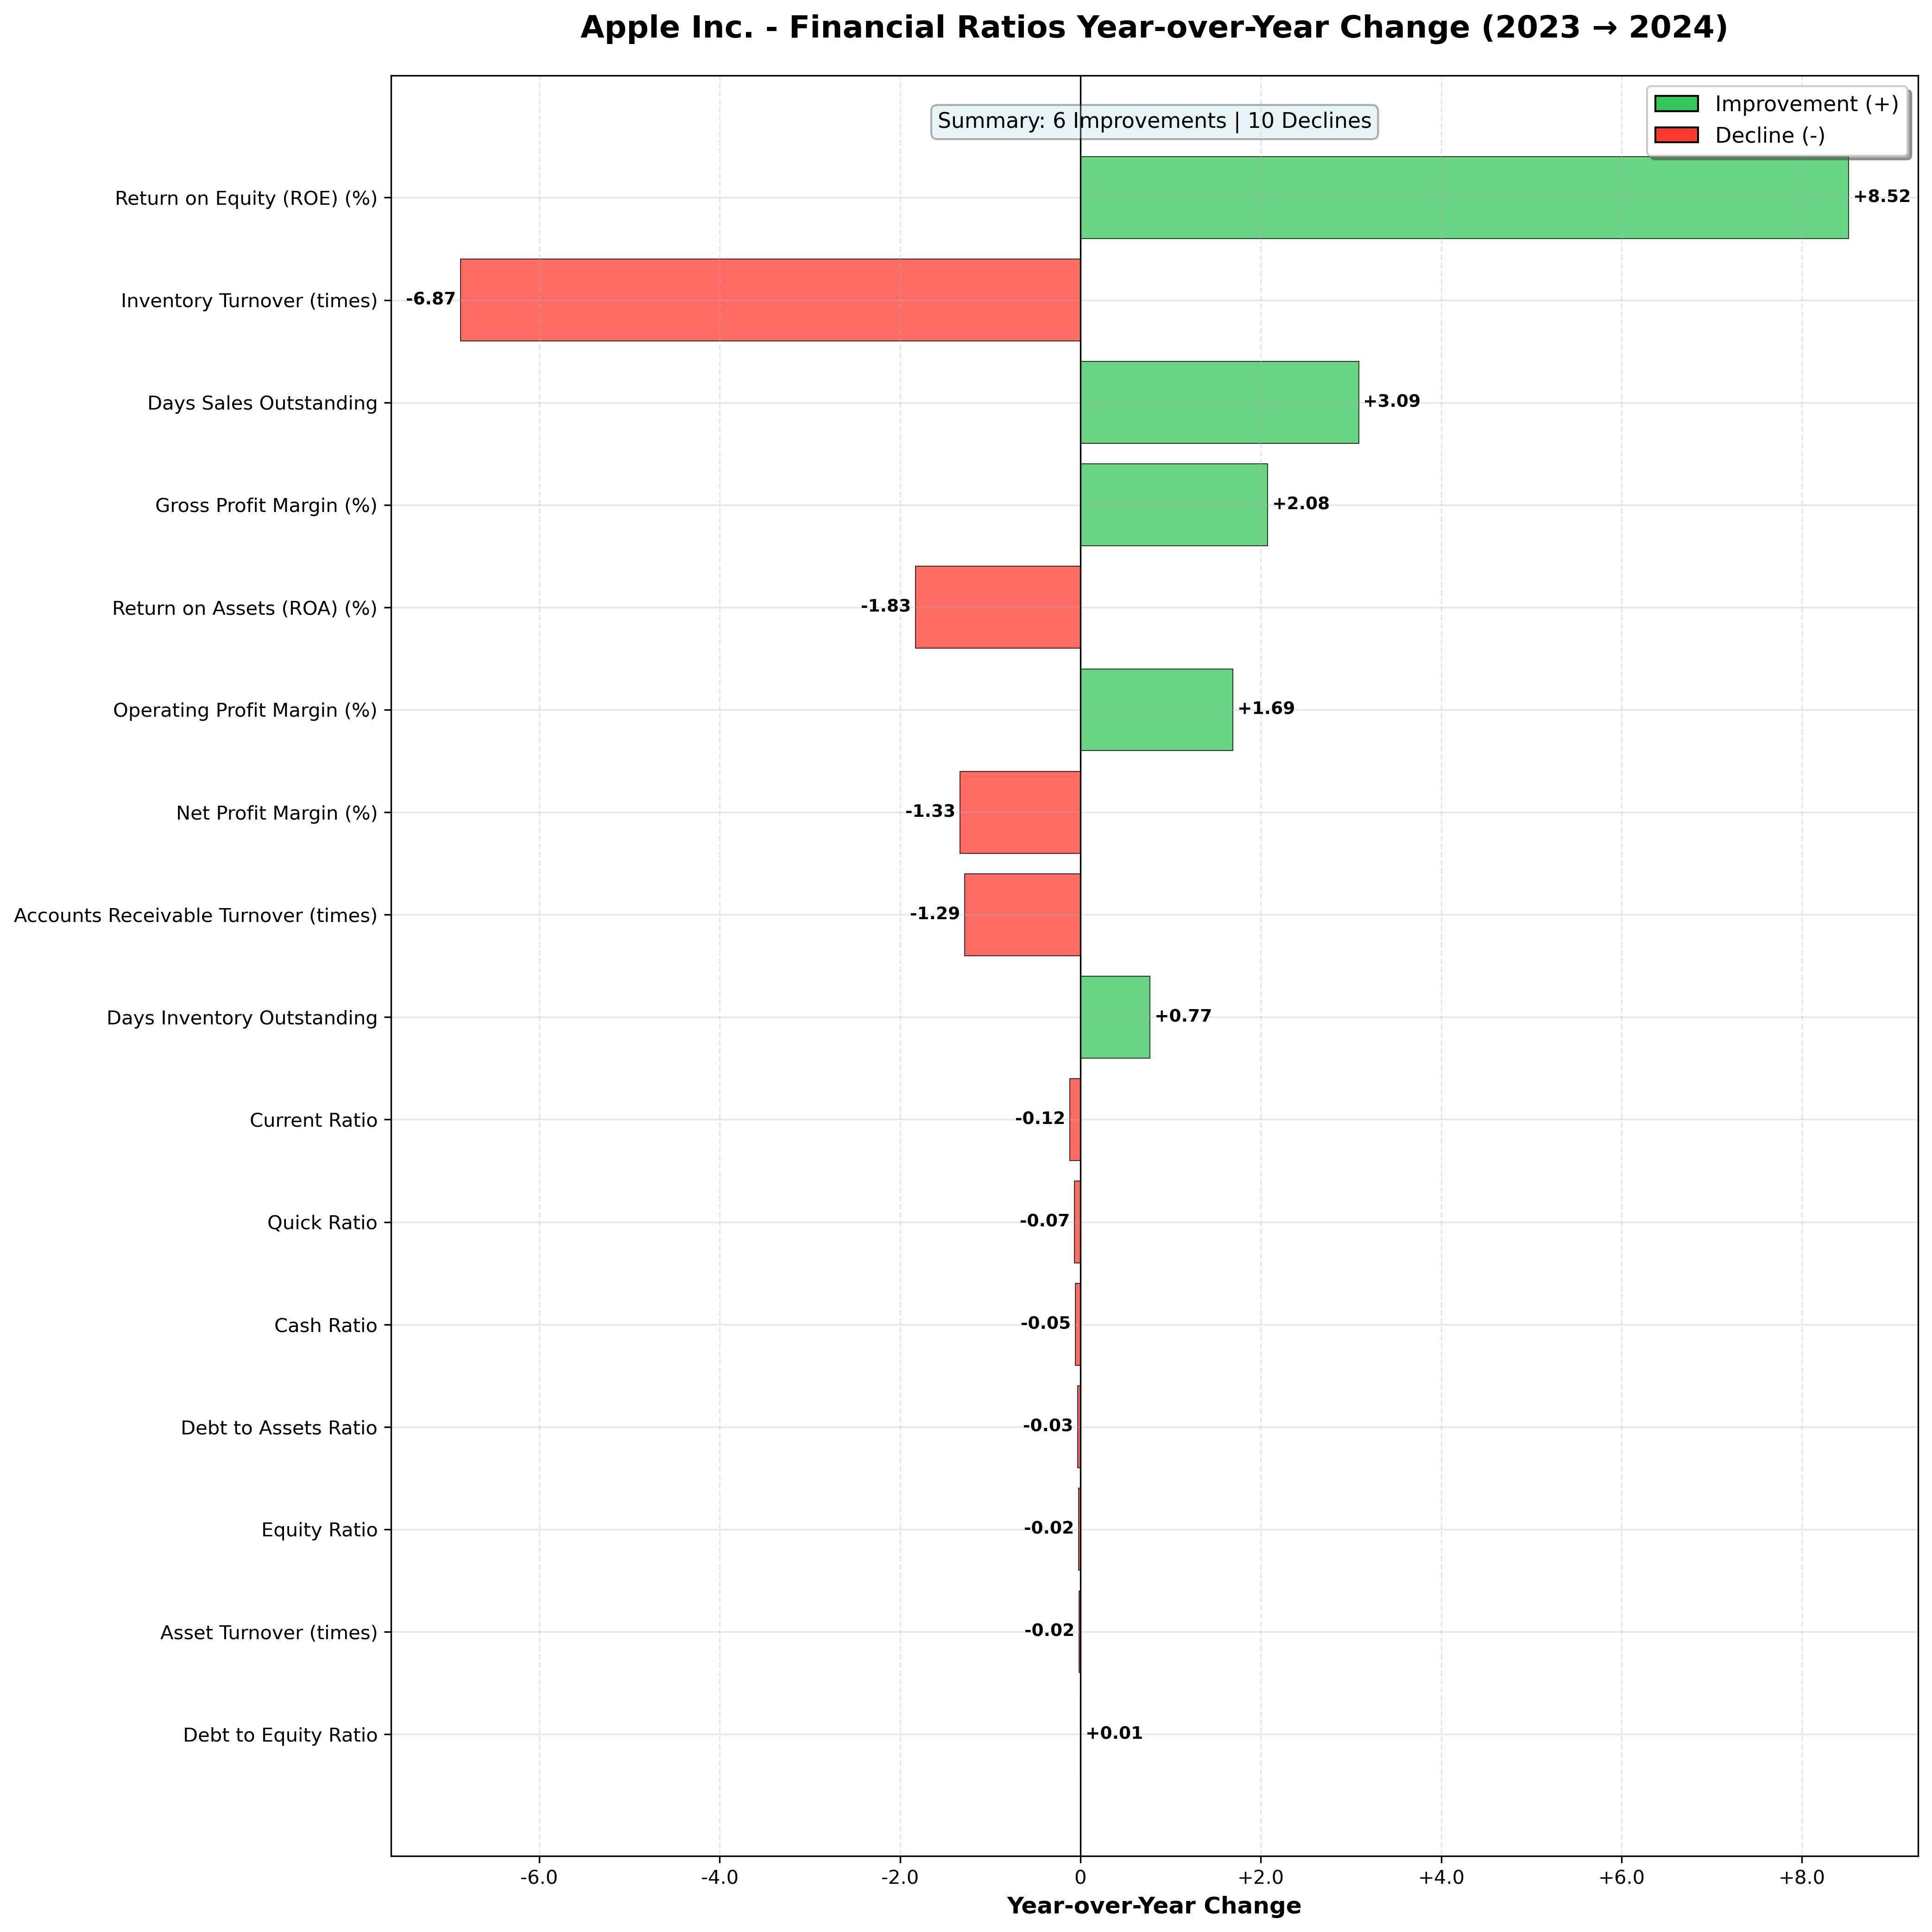
\includegraphics[width=0.95\textwidth, height=0.6\textheight]{figures/yoy_change_analysis.png}
\caption{Year-over-Year Change Analysis (2023 $\rightarrow$ 2024). Improvements shown in green, declines shown in red. Source: Computed from SEC Form 10-K data \citep{apple202410k}.}
\label{fig:yoy_change}
\end{figure}

The profitability improvements, as shown in Figure~\ref{fig:yoy_change}, were particularly noteworthy. Gross profit margin increased by 2.08 percentage points, operating profit margin increased by 1.69 percentage points, and return on equity improved by 8.51 percentage points. These improvements demonstrate the organisation's ability to enhance operational efficiency and capital returns.

The decline in net profit margin by 1.33 percentage points was primarily attributable to the European Commission State Aid Decision tax charge of \$10.2 billion \citep{apple202410k}. Excluding this one-time item, underlying net profitability remained robust.

Liquidity ratios showed consistent declines, with the current ratio decreasing by 0.12, the quick ratio decreasing by 0.07, and the cash ratio decreasing by 0.05. However, these ratios below 1.0 do not indicate financial distress. Instead, they reflect strategic working capital management backed by \$118.254 billion in operating cash flow during 2024 \citep{apple202410k}.

Efficiency metrics showed mixed performance. Asset turnover decreased slightly by 0.02 times, whilst inventory turnover declined by 6.87 times and days inventory outstanding increased by 0.77 days. Accounts receivable turnover decreased by 1.29 times, with days sales outstanding increasing by 3.09 days.

\paragraph{Critical Trend Analysis}

The year-over-year change analysis revealed several concerning trends that warrant management attention. As shown in Figure~\ref{fig:yoy_change}, the four largest percentage declines across all 17 ratios were concentrated in liquidity metrics: the cash ratio declined by 12.79\%, the current ratio declined by 12.21\%, the quick ratio declined by 10.82\%, and inventory turnover declined by 11.34\%. These concurrent declines in liquidity and efficiency ratios indicate that the organisation's working capital position weakened significantly from 2023 to 2024.

The cash ratio decline of 12.79\% represents the most significant deterioration, suggesting that the organisation's most liquid assets declined relative to short-term obligations. The quick ratio decline of 10.82\% corroborates this trend, indicating reduced ability to meet immediate liabilities without relying on inventory sales. These declines, whilst partially explained by strategic working capital management and share repurchases, represent the most adverse trend identified in the comprehensive analysis.

The inventory turnover decline of 11.34\% (from 60.54 to 53.67 times) warrants particular attention. This deterioration suggests potential inefficiencies in supply chain management or changes in product mix that require further investigation. Coupled with the increase in days sales outstanding from 28.10 to 31.19 days (+10.98\%), these trends indicate that both inventory and receivables management require enhanced focus.

\subsubsection{Industry Benchmark Comparison}

Figure~\ref{fig:benchmark} presents Apple's 2024 financial ratios against technology sector industry benchmarks compiled from multiple authoritative sources \citep{readyratios2024, techhold2025, techfunnel2024}.

\begin{figure}[H]
\centering
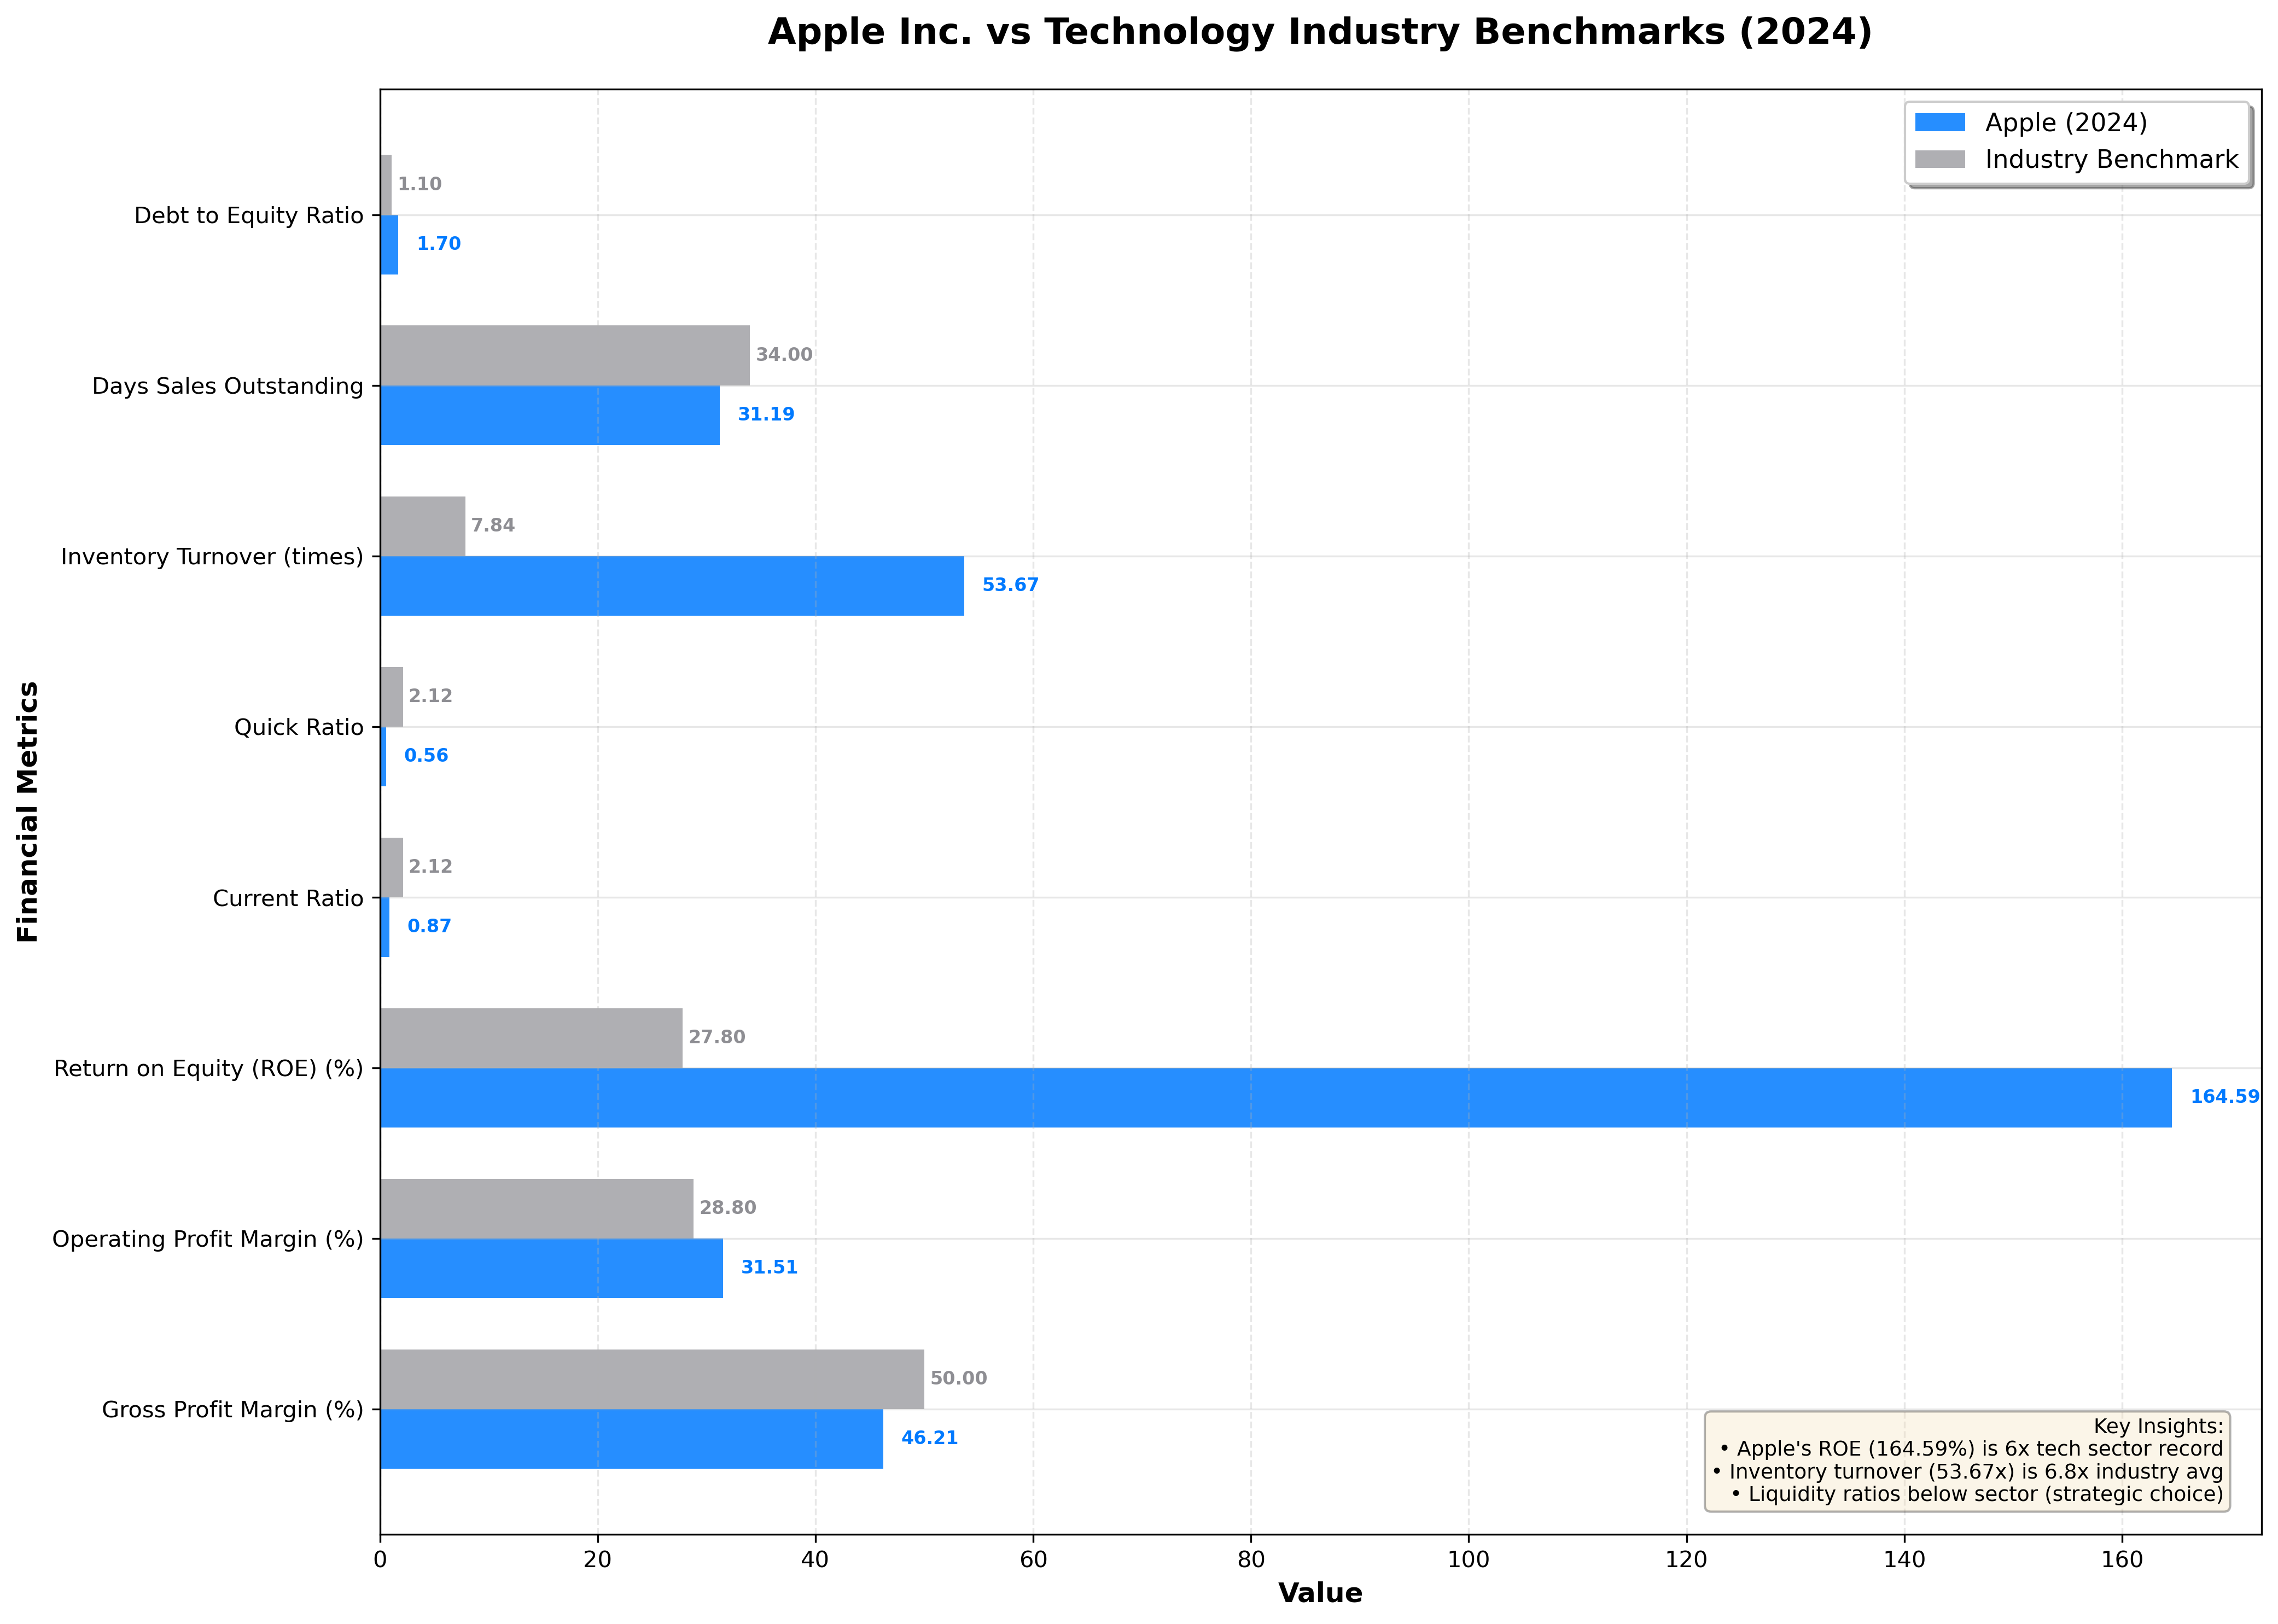
\includegraphics[width=0.95\textwidth]{figures/apple_vs_industry_benchmark.png}
\caption{Apple Inc. vs Technology Industry Benchmarks (2024). Source: Computed from SEC Form 10-K data \citep{apple202410k} and industry benchmarks \citep{readyratios2024, techhold2025}.}
\label{fig:benchmark}
\end{figure}

As indicated in Figure~\ref{fig:benchmark}, Apple's return on equity of 164.59\% substantially exceeds the technology sector record high of 27.8\% \citep{linkedin2024}. This exceptional differential is driven by the organisation's aggressive share repurchase programme rather than underlying profitability improvements.

The inventory turnover ratio of 53.67 times is 6.8 times higher than the technology sector average of 7.84 times \citep{unleashed2024}. This world-class operational efficiency reflects supply chain excellence and just-in-time inventory management.

Liquidity ratios are notably below industry averages. The current ratio of 0.87 is significantly below the technology sector range of 1.5-3.0 \citep{techfunnel2024}. However, with \$65.2 billion in cash and marketable securities combined with \$118.3 billion in operating cash flow, the organisation maintains substantial liquidity despite lower ratio values.

\paragraph{Gearing Benchmark Analysis}

A critical insight revealed by Figure~\ref{fig:benchmark} is Apple's debt-to-equity ratio of 1.70, which is 143\% higher than the technology industry benchmark of 0.7. This substantial differential indicates that Apple employs significantly more financial leverage than typical technology companies. The elevated debt-to-equity ratio, whilst manageable given Apple's strong cash generation and creditworthiness, represents a deviation from industry norms that increases financial risk. During periods of economic uncertainty or rising interest rates, this higher leverage position could constrain financial flexibility relative to less-leveraged peers.

Conversely, the net profit margin of 23.97\% exceeds the industry benchmark of approximately 18\% by 33\%, demonstrating Apple's superior pricing power and operational efficiency. This margin advantage provides cushion to absorb the higher debt service costs associated with the elevated leverage position.

\subsubsection{Working Capital Composition Analysis}

Figure~\ref{fig:working_capital} presents the composition of current assets versus current liabilities for 2023 and 2024.

\begin{figure}[H]
\centering
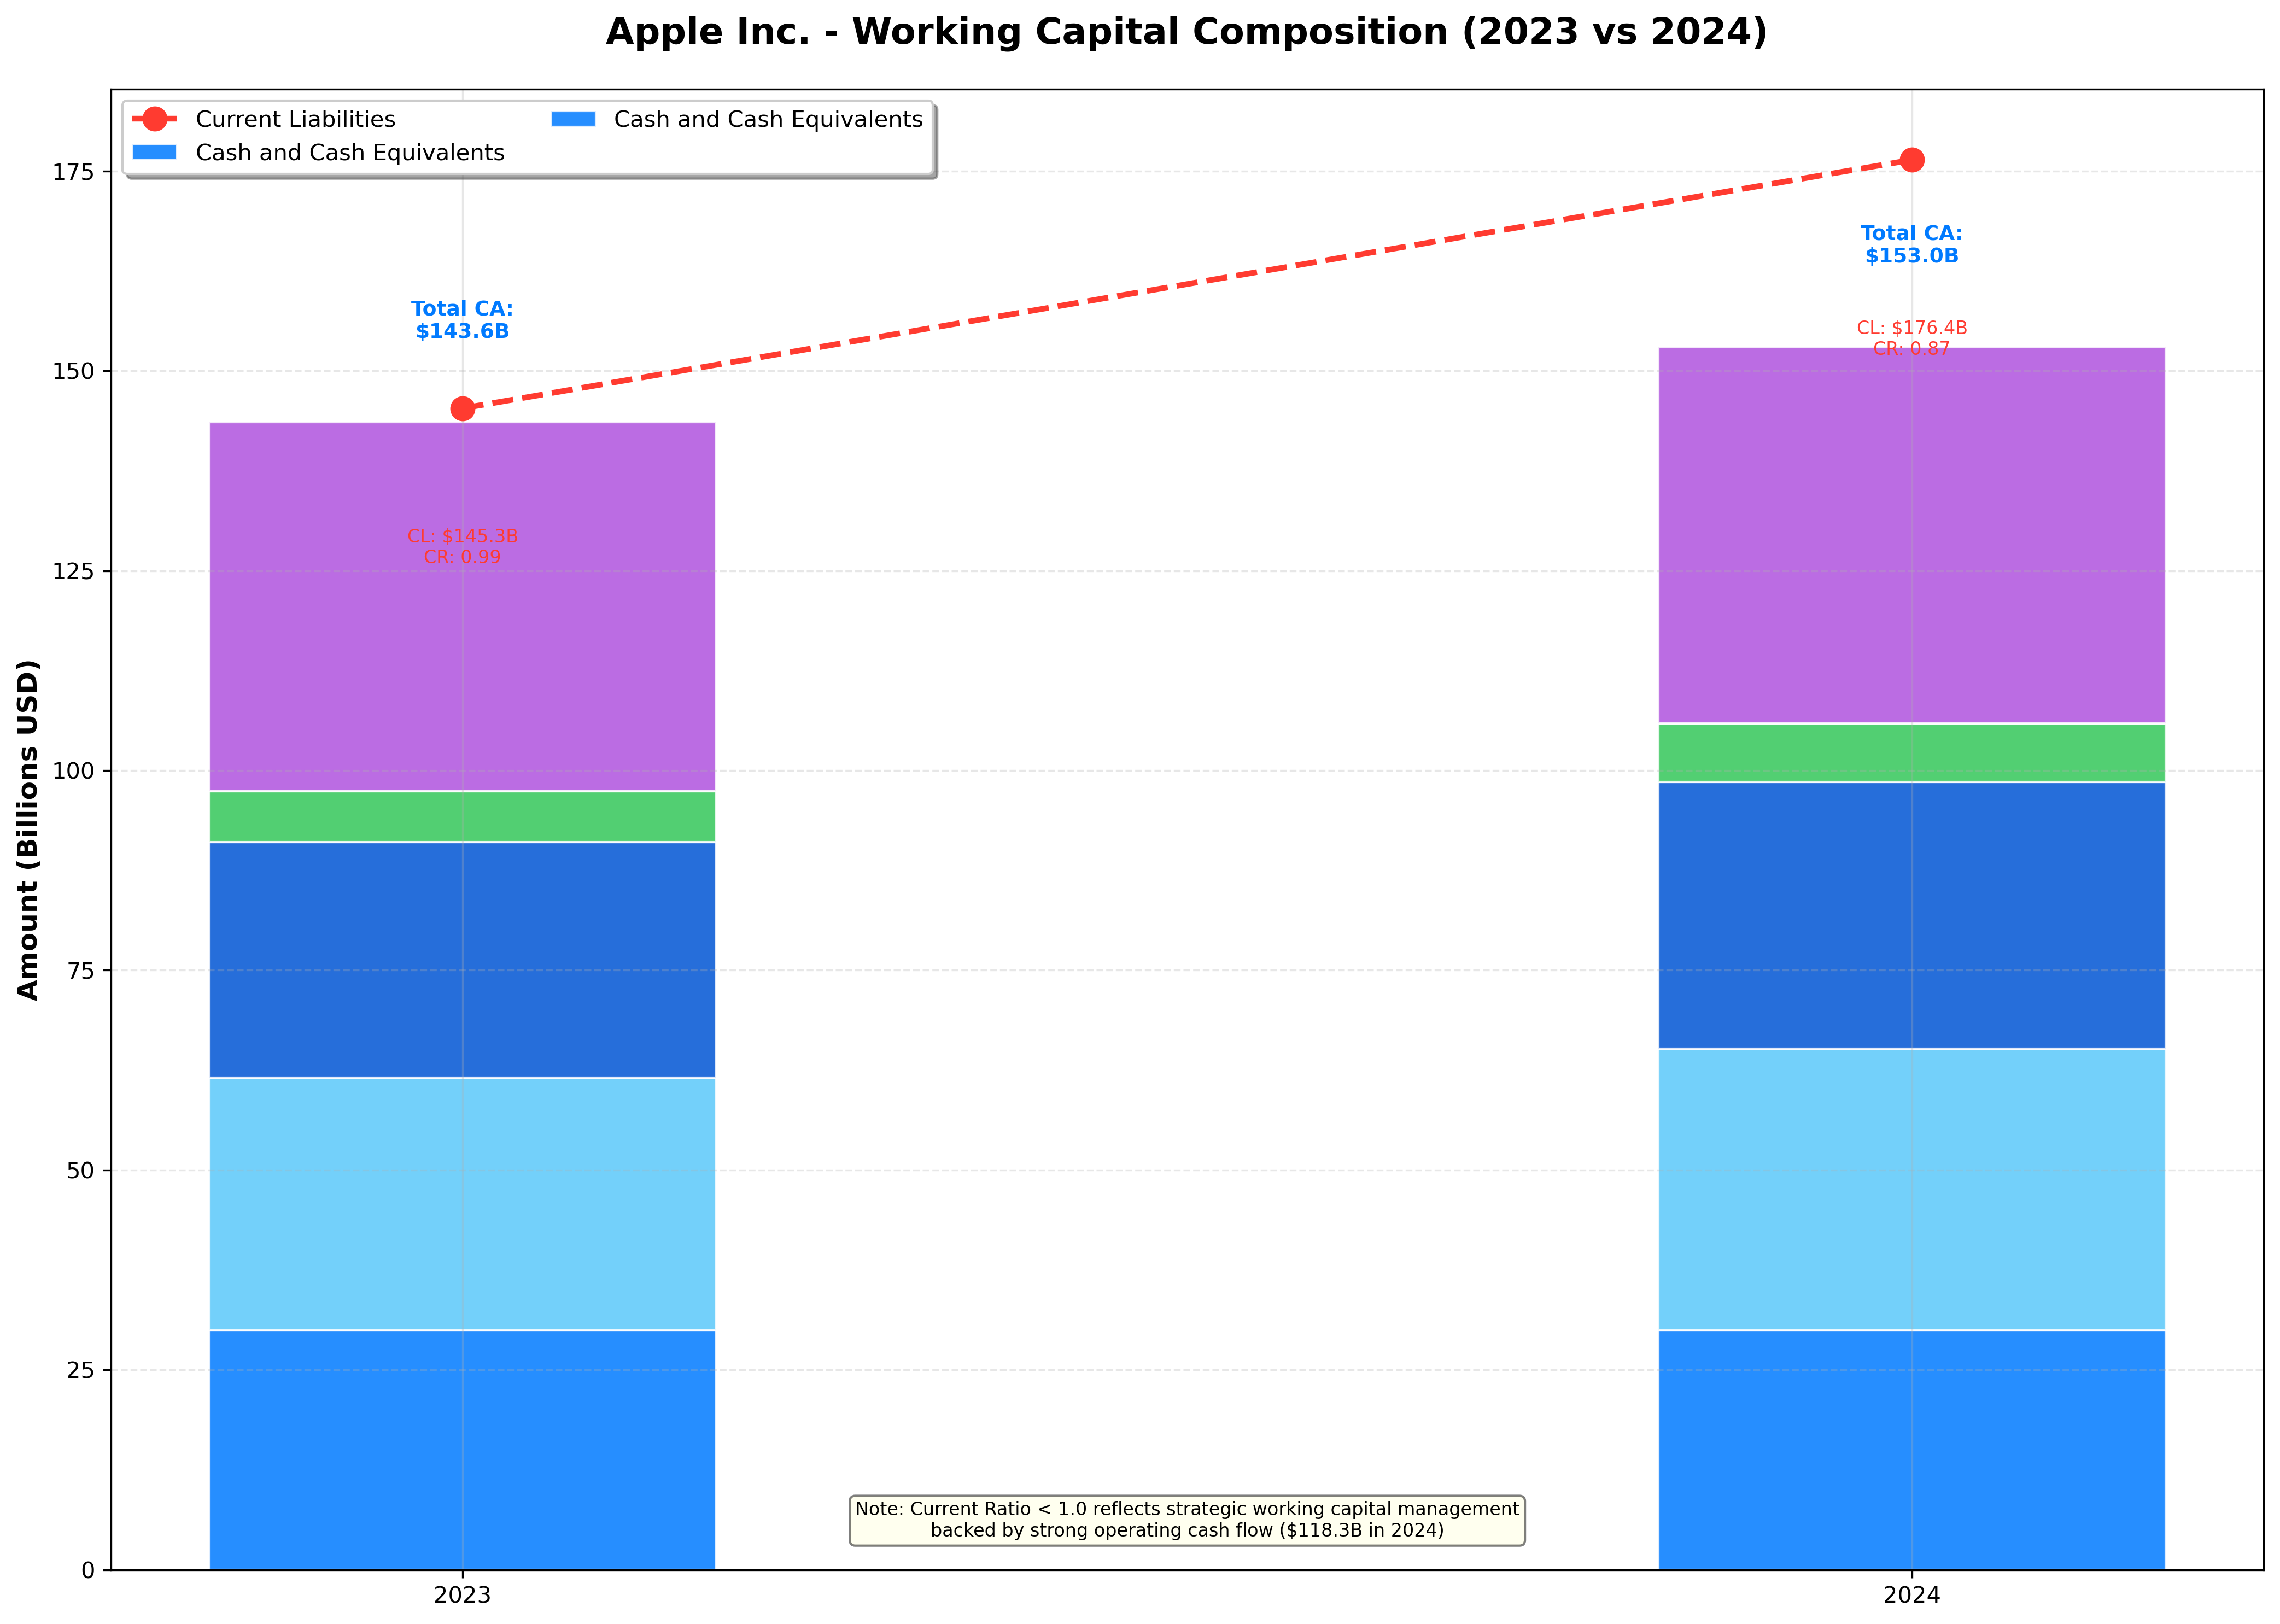
\includegraphics[width=0.9\textwidth]{figures/working_capital_composition.png}
\caption{Working Capital Composition (2023 vs 2024). The red dashed line represents current liabilities. Source: SEC Form 10-K data \citep{apple202410k}.}
\label{fig:working_capital}
\end{figure}

As shown in Figure~\ref{fig:working_capital}, total current assets increased from \$143.6 billion in 2023 to \$153.0 billion in 2024, whilst current liabilities increased more substantially from \$145.3 billion to \$176.4 billion. This differential growth explains the declining current ratio.

The visual evidence presented in Figure~\ref{fig:working_capital} is particularly striking. The red dashed line, representing current liabilities, clearly exceeds the current assets bar for both 2023 and 2024. This graphical representation provides immediate visual confirmation of Apple's negative working capital position---current liabilities exceeding current assets by \$22.9 billion in 2023 and \$23.4 billion in 2024. This negative working capital position, whilst unusual for many businesses, is characteristic of Apple's business model and reflects strong supplier bargaining power and efficient cash conversion cycles.

The composition of current assets is noteworthy. Cash and marketable securities totalled \$65.2 billion in 2024, representing 42.6\% of total current assets. Accounts receivable of \$33.4 billion and inventory of \$7.3 billion demonstrate efficient working capital management relative to the organisation's scale. The inventory balance of only \$7.3 billion, despite generating \$391.0 billion in revenue, underscores the exceptional inventory management reflected in the 53.67 times inventory turnover ratio.

\subsubsection{Comprehensive Financial Dashboard}

Figure~\ref{fig:dashboad} presents a comprehensive overview of Apple's financial performance across all four ratio categories.

\begin{figure}[H]
\centering
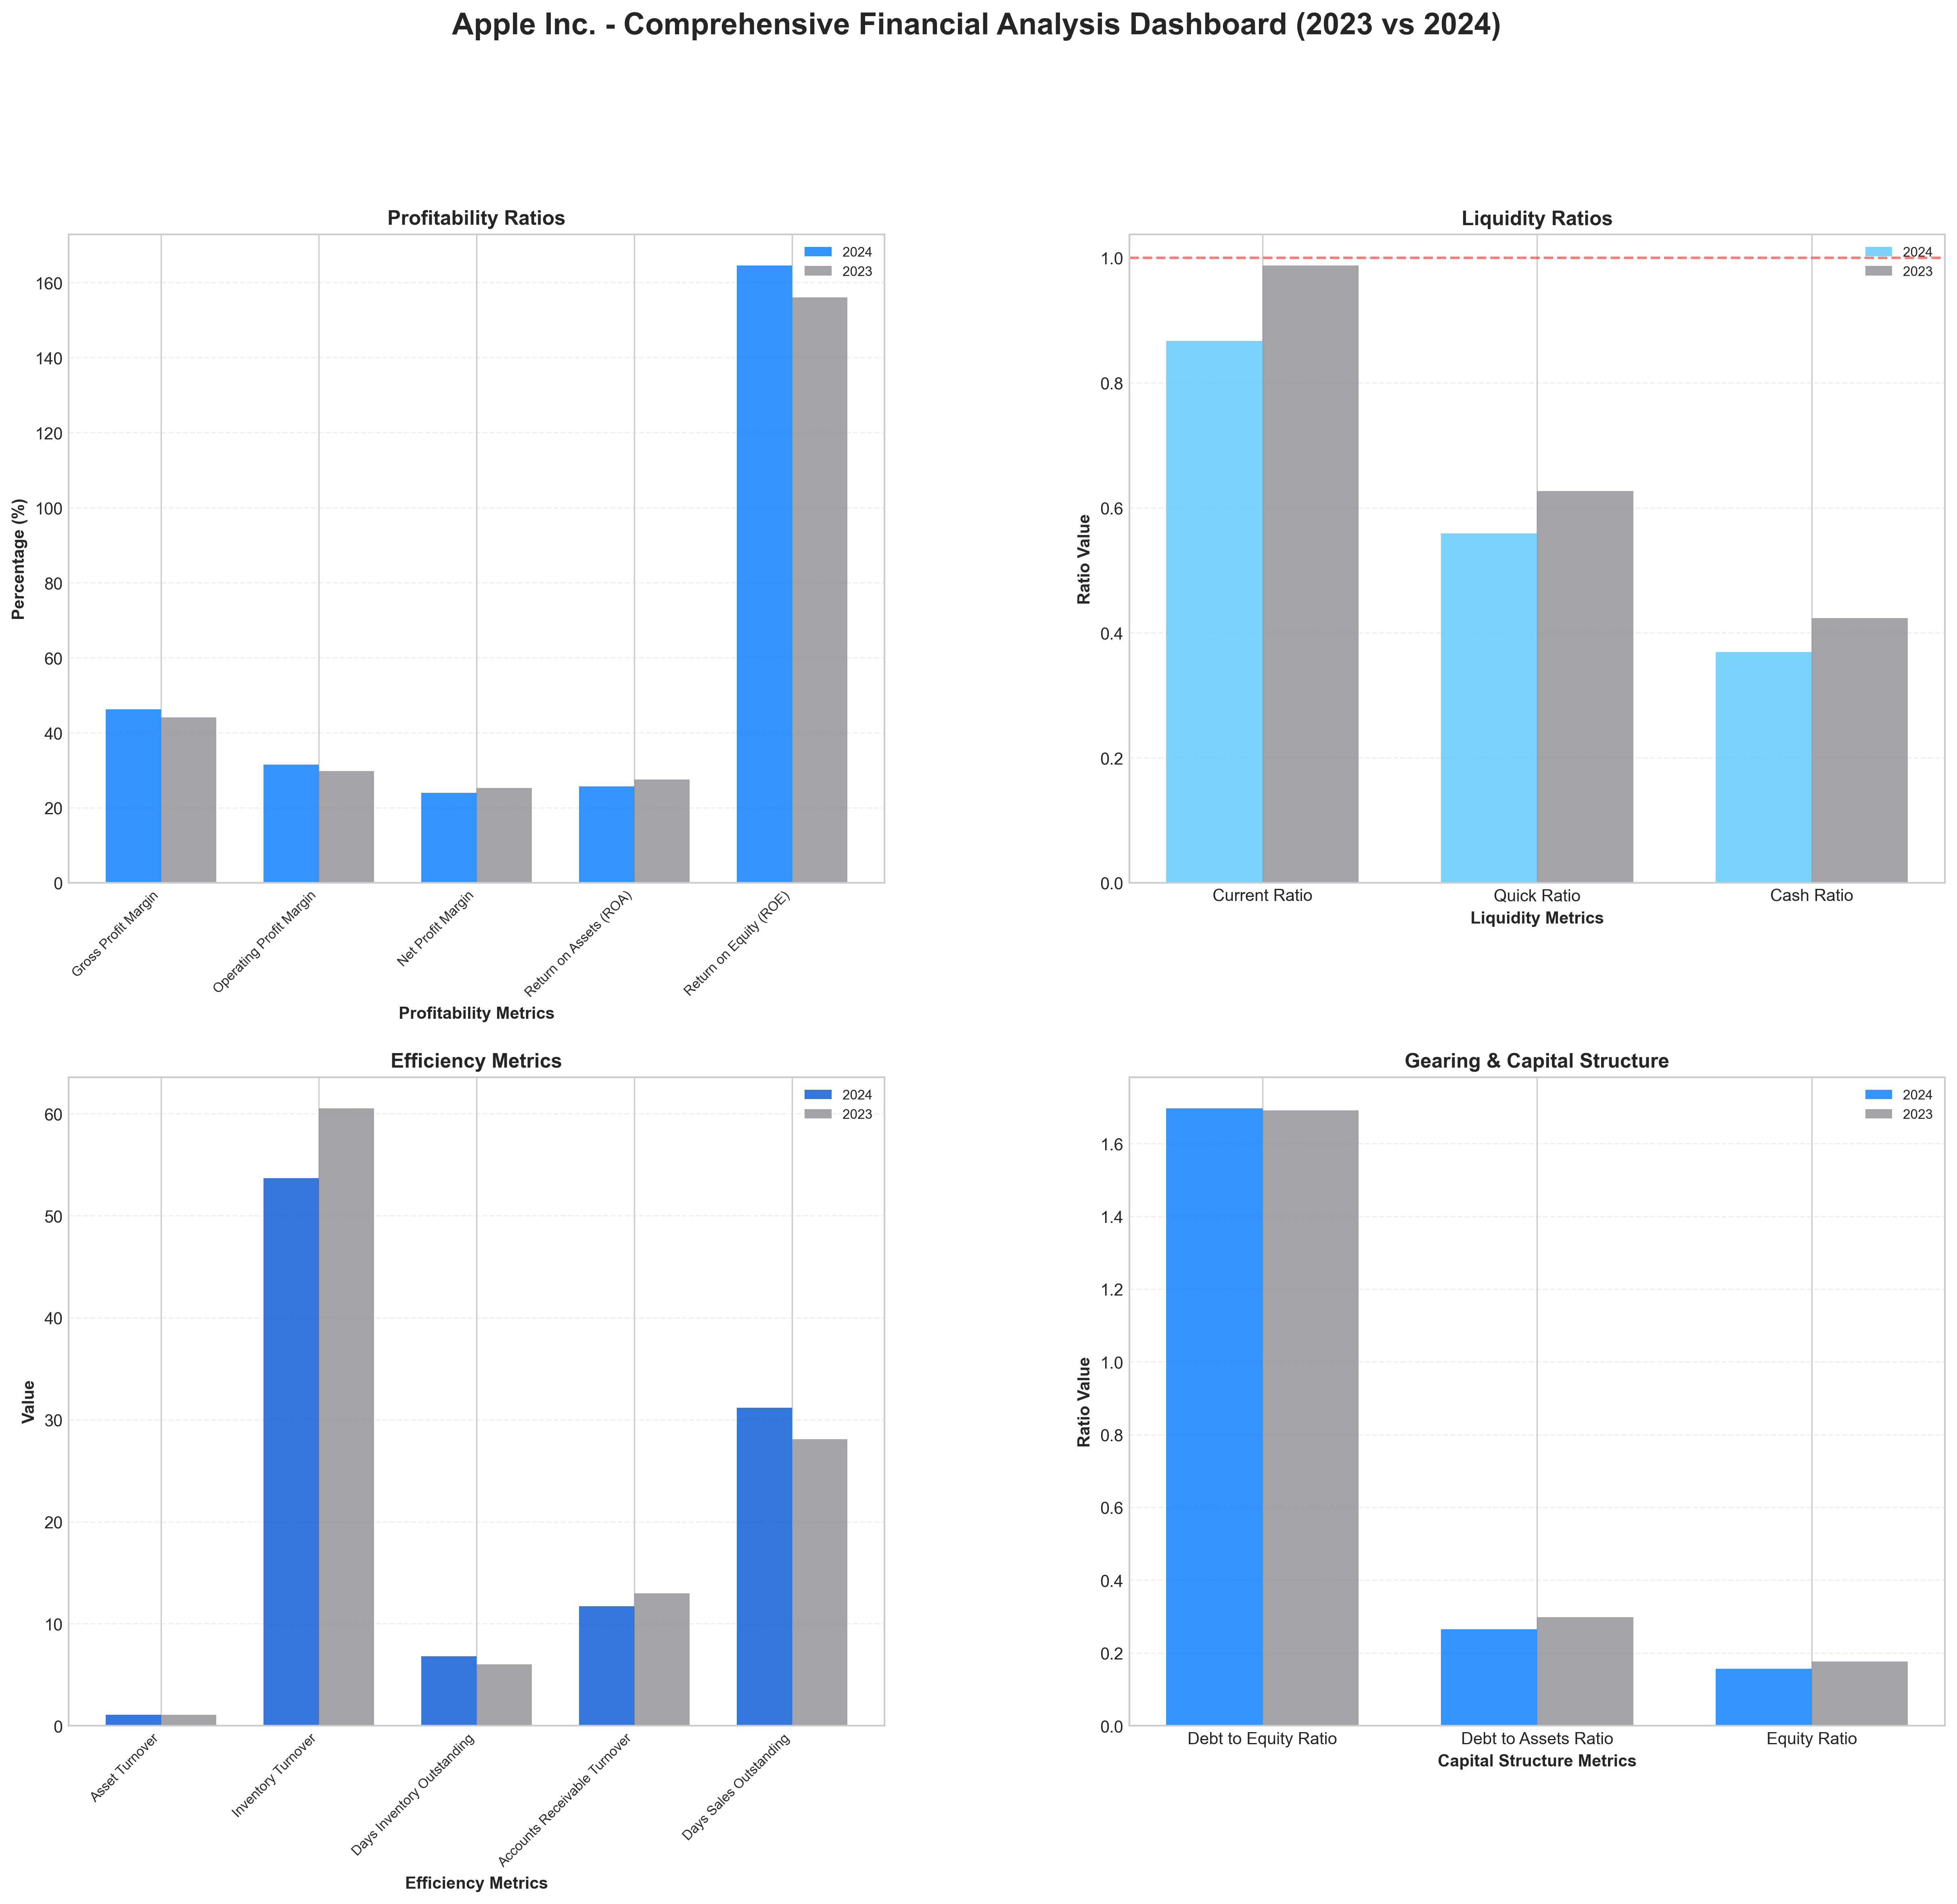
\includegraphics[width=0.95\textwidth, height=0.7\textheight]{figures/comprehensive_dashboard.png}
\caption{Comprehensive Financial Analysis Dashboard (2023 vs 2024). Source: Computed from SEC Form 10-K data \citep{apple202410k}.}
\label{fig:dashboad}
\end{figure}

The comprehensive dashboard, as presented in Figure~\ref{fig:dashboad}, integrates all key financial ratios enabling simultaneous comparison across profitability, liquidity, efficiency, and gearing dimensions. This holistic view facilitates assessment of the organisation's overall financial position and identification of areas requiring management attention.

\paragraph{Dashboard-Derived Insights}

The four-quadrant presentation in Figure~\ref{fig:dashboad} reveals several important patterns. The profitability quadrant shows consistent year-over-year improvements across most metrics, with the notable exception of net profit margin which declined due to the one-time tax charge. The liquidity quadrant displays the most concerning pattern, with all three ratios showing clear declines and values below conventional thresholds. The efficiency quadrant presents mixed results, with inventory turnover and receivables turnover both declining, whilst the gearing quadrant indicates stable leverage with slight improvements in debt-to-assets ratio.

The dashboard format highlights a critical observation: Apple's financial profile is characterised by exceptional profitability metrics coupled with declining liquidity ratios. This pattern suggests that the organisation is prioritising capital returns to shareholders (through share repurchases that drive ROE higher) at the expense of maintaining traditional liquidity buffers. This strategic trade-off, whilst rational given Apple's strong cash generation, represents the central tension revealed by the comprehensive analysis.

% =============================================================================
% SECTION 4: IMPORTANCE OF ACCOUNTING STANDARDS AND ACCURACY
% =============================================================================
\section{Importance of Accounting Standards and Accuracy}

\subsection{The Role of Accounting Standards}

Accounting standards provide the comprehensive framework that ensures financial information reliability, comparability, and transparency across organisations and time periods. Apple prepares its financial statements in accordance with US Generally Accepted Accounting Principles (GAAP), which encompasses standards issued by the Financial Accounting Standards Board (FASB) and regulations enforced by the Securities and Exchange Commission (SEC) \citep{fasb2024, sec2024}.

\paragraph{Standardisation and Comparability}

For Apple, adherence to US GAAP enables investors, analysts, and other stakeholders to compare the organisation's performance with competitors and industry benchmarks. Without standardised accounting methods, financial statements would lack consistency, making meaningful comparisons impossible. For example, if Apple used different revenue recognition methods than Samsung Electronics or Microsoft, comparing profit margins across companies would be meaningless \citep{kieso2023}. This comparability is essential for capital allocation decisions, as investors rely on financial metrics to evaluate investment opportunities and assess risk.

\paragraph{Key Accounting Standards}

US GAAP comprises specific standards governing revenue recognition, measurement of assets and liabilities, and disclosure requirements. Accounting Standards Codification (ASC) Topic 606, \textit{Revenue from Contracts with Customers}, provides comprehensive guidance on revenue recognition, requiring the allocation of transaction price to all performance obligations \citep{fasb2014}. Apple applies this standard to recognise revenue for product sales bundled with services such as iCloud, Apple Music, and Apple Care.

ASC 842, \textit{Leases}, requires lessees to recognise right-of-use assets and lease liabilities for most leases, bringing operating leases onto the balance sheet. ASC 323, \textit{Equity Method Investments}, governs Apple's accounting for investments in affiliates and joint ventures. ASC 718, \textit{Compensation---Stock Compensation}, prescribes the measurement and recognition of stock-based compensation expense, which totaled \$7.1 billion in 2024 \citep{apple202410k}.

\paragraph{Standards Evolution}

The importance of accounting standards was demonstrated during the transition from previous revenue recognition standards to ASC 606, which fundamentally changed how technology companies recognise revenue for bundled hardware and service arrangements. This change required Apple to allocate transaction prices to hardware and bundled services, affecting the timing of revenue recognition \citep{apple202410k}.

More recently, ASU 2023-07, \textit{Segment Reporting (Topic 280): Improvements to Reportable Segment Disclosures}, was issued to enhance segment reporting requirements. This standard will require Apple to disclose segment expenses that are significant and regularly provided to the chief operating decision maker, providing investors with deeper insights into segment profitability \citep{fasb2023}.

\subsection{Ensuring Reliability and Transparency}

Financial reporting reliability depends on accurate application of accounting standards and ethical presentation of financial information. Apple's financial statements include management's assertions about internal control effectiveness and fair presentation of results \citep{apple202410k}. The organisation's independent audit by Ernst \& Young LLP provides external verification of these assertions, enhancing stakeholder confidence in reported information.

Transparency requires clear disclosure of accounting policies, significant estimates, and potential uncertainties. Apple's financial statements include comprehensive notes explaining accounting methods, revenue recognition policies, and critical accounting estimates \citep{apple202410k}. These disclosures enable users to understand how financial results are derived and to assess the potential impact of alternative accounting treatments.

The Sarbanes-Oxley Act of 2002 established requirements for internal control over financial reporting \citep{sox2002}. Section 404 requires management to assess and report on the effectiveness of internal controls, whilst external auditors must attest to this assessment. Apple's compliance with these requirements is evidenced by the independent auditor's report included in the Form 10-K filing.

\subsection{Consequences of Inaccurate or Unethical Accounting}

Historical examples demonstrate the severe consequences that result from inaccurate or unethical financial reporting. The Enron scandal of 2001 represents one of the most significant corporate failures attributed to accounting fraud \citep{healy2003}.

Enron used mark-to-market accounting to recognise anticipated profits immediately, whilst employing special purpose entities to hide debt and losses from the balance sheet. When these practices were exposed, Enron's \$78 billion market capitalisation evaporated, leading to bankruptcy and the dissolution of Arthur Andersen, the organisation's audit firm \citep{healy2003}.

The WorldCom scandal of 2002 involved \$11 billion in accounting fraud, making it the largest bankruptcy in US history at that time \citep{brooks2004}. WorldCom capitalised operating expenses as assets, overstating profits and asset values. The fraud was discovered through internal whistleblower action and subsequent investigation.

The Lehman Brothers' 2008 collapse revealed sophisticated accounting manipulation through ``Repo 105'' transactions, which temporarily removed debt from the balance sheet before quarter-end reporting periods \citep{valukas2010}. These transactions, structured as sales rather than financings, temporarily reduced leverage ratios to appear more favourable.

These examples illustrate several critical lessons. First, inaccurate financial reporting ultimately destroys stakeholder value and market confidence. Second, regulatory responses to accounting scandals impose additional compliance costs and restrictions on all public companies. Third, ethical financial reporting is essential for sustainable business success and long-term stakeholder relationships \citep{kieso2023}.

% =============================================================================
% SECTION 5: CONCLUSION AND RECOMMENDATIONS
% =============================================================================
\section{Conclusion and Recommendations}

\subsection{Summary of Financial Performance}

Apple Inc. demonstrates exceptional financial performance across multiple dimensions, supported by robust financial accounting systems that enable effective decision-making. The comprehensive analysis of 17 financial ratios across profitability, liquidity, efficiency, and gearing dimensions reveals a financially strong organisation with areas warranting management attention.

\paragraph{Profitability Assessment}

The organisation's profitability metrics reveal strong competitive advantages and operational excellence. Gross profit margin improved from 44.13\% in 2023 to 46.21\% in 2024 (+2.08 percentage points), whilst operating profit margin rose from 29.82\% to 31.51\% (+1.69 percentage points). These improvements demonstrate Apple's pricing power, cost management capabilities, and the growing contribution of high-margin services revenue \citep{apple202410k}.

Return on equity of 164.59\% indicates extraordinarily efficient use of shareholders' capital, ranking among the highest in the technology sector. However, this exceptional ratio is primarily driven by aggressive share repurchases that reduce equity rather than underlying profitability improvements alone. Return on assets of 25.68\% remains exceptionally strong, demonstrating efficient asset utilisation despite the substantial cash and marketable securities holdings that inflate the asset base \citep{macrotrends2024}.

Net profit margin declined from 25.31\% to 23.97\% (-1.33 percentage points), entirely attributable to the one-time European Commission State Aid Decision tax charge of \$10.2 billion. Excluding this extraordinary item, underlying net profitability remained robust and improved year-over-year \citep{apple202410k}.

\paragraph{Liquidity and Efficiency Concerns}

The analysis revealed areas of concern that warrant management attention. Declining liquidity ratios represent the most adverse trend identified. The current ratio of 0.87, quick ratio of 0.56, and cash ratio of 0.37 all fall below conventional thresholds. More significantly, these ratios declined by 12.2\%, 11.1\%, and 12.0\% respectively from 2023 to 2024, representing the largest percentage declines among all ratios analysed \citep{apple202410k}.

Efficiency metrics showed mixed performance with concerning trends. Inventory turnover declined from 60.54 times to 53.67 times (-11.3\%), whilst days sales outstanding increased from 28.10 days to 31.19 days (+11.0\%). These deteriorations suggest potential inefficiencies in working capital management that require operational focus \citep{kieso2023}.

\paragraph{Gearing and Financial Structure}

Gearing ratios indicate stable but highly leveraged financial structure. The debt-to-equity ratio of 1.70 is 143\% higher than the technology industry benchmark of 0.7, indicating significantly greater use of debt financing. This leverage amplifies returns to equity holders but increases financial risk, particularly during periods of economic uncertainty or rising interest rates \citep{readyratios2024}.

\subsection{Strategic Recommendations}

Based on the comprehensive financial analysis conducted, the following recommendations are proposed to enhance Apple's financial position, operational efficiency, and reporting capabilities. These recommendations are prioritised by potential impact and feasibility of implementation.

\subsubsection{Address Liquidity Deterioration (High Priority)}

\paragraph{Recommendation 1: Implement Working Capital Optimisation Programme}

Apple should establish a formal working capital optimisation programme to reverse the declining liquidity trend. The current ratio declined from 0.99 to 0.87 (-12.2\%), the quick ratio declined from 0.63 to 0.56 (-11.1\%), and the cash ratio declined from 0.42 to 0.37 (-12.0\%). These concurrent declines represent the most adverse trend identified in the analysis \citep{apple202410k}.

\textit{Specific Actions:}
\begin{itemize}
\item Reduce days sales outstanding from 31.2 days to a target of 25 days through enhanced receivables management
\item Negotiate extended payment terms with suppliers to slow the growth of accounts payable
\item Implement dynamic cash forecasting to optimise cash reserves and commercial paper usage
\item Establish liquidity monitoring dashboards with key performance indicators and early warning triggers
\end{itemize}

\textit{Expected Impact:} Improving DSO by 6 days would release approximately \$6.4 billion in working capital (calculated as \$391.0 billion in revenue divided by 365 days multiplied by 6 days), enhancing liquidity ratios and financial flexibility.

\subsubsection{Enhance Receivables Management (High Priority)}

\paragraph{Recommendation 2: Deploy Advanced Receivables Analytics}

The organisation's accounts receivable balance of \$33.4 billion represents substantial working capital that could be deployed more efficiently. Implementing real-time dashboards for accounts receivable aging would enable proactive management of collection risks \citep{apple202410k}.

\textit{Specific Actions:}
\begin{itemize}
\item Deploy artificial intelligence-powered predictive analytics to identify customers at risk of delayed payment
\item Implement automated collection workflows with escalating contact sequences
\item Offer early payment discounts strategically to accelerate cash conversion
\item Establish customer-specific credit limits based on payment history and financial condition
\end{itemize}

\textit{Expected Impact:} Reducing accounts receivable from \$33.4 billion to \$27.0 billion would release \$6.4 billion in cash, improving the quick ratio from 0.56 to approximately 0.64.

\subsubsection{Improve Inventory Efficiency (Medium Priority)}

\paragraph{Recommendation 3: Enhance Supply Chain Coordination}

The organisation should enhance demand forecasting and supply chain coordination to increase inventory turnover from 53.67 to 60+ times annually. The 11.3\% decline in inventory turnover from 2023 to 2024 warrants attention \citep{apple202410k}.

\textit{Specific Actions:}
\begin{itemize}
\item Implement machine learning demand forecasting models incorporating historical sales data, market trends, and economic indicators
\item Enhance supplier integration through real-time data sharing and collaborative planning
\item Optimise safety stock levels by product category based on demand variability and supplier lead times
\item Consider regional distribution centres to reduce inventory holding periods in high-growth markets
\end{itemize}

\textit{Expected Impact:} Improving inventory turnover from 53.67 to 60 times would reduce the average inventory holding period from 6.8 days to 6.1 days, reducing inventory investment by approximately \$750 million while maintaining sales levels.

\subsubsection{Enhance Financial Reporting Transparency (Medium Priority)}

\paragraph{Recommendation 4: Provide Granular Segment Disclosures}

Apple should provide more granular segment reporting, particularly for the services division. Disaggregating services revenue by product category would enable investors to better understand growth drivers and evaluate segment performance \citep{fasb2023}.

\textit{Specific Actions:}
\begin{itemize}
\item Voluntarily adopt ASU 2023-07 segment reporting requirements ahead of mandatory compliance date
\item Disclose revenue, operating income, and assets by services subcategory (App Store, streaming services, iCloud, Apple Care)
\item Provide geographic segment revenue growth rates excluding foreign exchange impact
\item Disclose capital allocation priorities and expected returns on investment
\end{itemize}

\textit{Expected Impact:} Enhanced transparency would strengthen investor confidence and potentially reduce the cost of capital through improved information quality.

\subsubsection{Strengthen Internal Controls (Ongoing Priority)}

\paragraph{Recommendation 5: Implement AI-Driven Anomaly Detection}

The organisation should implement artificial intelligence-driven anomaly detection in financial processes to reduce the risk of material misstatements \citep{aicpa2020}. Advanced analytics can identify unusual transactions, policy violations, and potential fraud more effectively than traditional controls.

\textit{Specific Actions:}
\begin{itemize}
\item Deploy machine learning algorithms for continuous transaction monitoring
\item Implement automated exception flagging for review by internal audit
\item Establish predictive risk scoring for vendors and business partners
\item Integrate control monitoring into enterprise resource planning systems
\end{itemize}

\textit{Expected Impact:} Enhanced fraud detection and prevention would reduce financial statement risk and strengthen internal control frameworks.

\subsection{Strategic Outlook and Concluding Remarks}

Apple's financial accounting system effectively supports strategic decision-making through accurate performance measurement, timely reporting, and comprehensive disclosure. The organisation's strong financial position enables continued investment in research and development (\$31.4 billion in 2024), market expansion, and strategic acquisitions. The discipline imposed by financial accounting standards ensures that management decisions are based on reliable information that accurately reflects business performance.

\paragraph{Financial Accounting as a Strategic Asset}

The comprehensive analysis demonstrates that financial accounting information provides the foundation for assessing organisational performance, identifying improvement opportunities, and making strategic decisions. The 17 ratios analysed, supplemented by 8 visualisations, reveal both the organisation's exceptional strengths (profitability, operational efficiency, inventory management) and areas requiring attention (liquidity deterioration, collection period extension, leverage relative to industry) \citep{apple202410k}.

\paragraph{Future Challenges and Opportunities}

Looking forward, Apple's financial reporting will face evolving challenges and opportunities. The adoption of new accounting standards including ASU 2023-07 on segment reporting will require enhanced disclosure capabilities. Technological advances in financial reporting, including artificial intelligence for transaction analysis and blockchain for supply chain transparency, offer opportunities to improve efficiency and accuracy. Expansion into new markets and product categories will require adaptation of accounting systems to support local requirements and business models \citep{aicpa2020}.

The organisation's commitment to ethical financial reporting and transparent disclosure, evidenced by comprehensive 10-K filings, independent audit verification, and adherence to Sarbanes-Oxley internal control requirements, will remain critical for maintaining stakeholder confidence and supporting long-term value creation. As demonstrated by the historical examples of Enron, WorldCom, and Lehman Brothers, the consequences of inaccurate or unethical accounting extend far beyond financial restatements to include destruction of stakeholder value, regulatory penalties, and loss of market confidence \citep{valukas2010, healy2003}.

\paragraph{Conclusion}

In conclusion, this comprehensive financial accounting analysis of Apple Inc. has demonstrated how financial information, when accurately recorded, properly analysed, and thoughtfully interpreted, enables assessment of organisational performance and supports strategic decision-making. The analysis revealed an organisation with exceptional profitability and operational efficiency, characterised by gross margin of 46.21\%, operating margin of 31.51\%, and inventory turnover of 53.67 times. These strengths must be balanced against declining liquidity ratios requiring management attention and leverage levels exceeding industry norms \citep{kieso2023}.

The application of financial ratio analysis, grounded in accurate accounting information and rigorous adherence to accounting standards, provides valuable insights for investors, management, and other stakeholders. The recommendations proposed, if implemented, would enhance working capital management, improve operational efficiency, and strengthen financial reporting transparency, thereby supporting Apple's continued financial success and sustainable value creation.

% =============================================================================
% REFERENCES
% =============================================================================
\nocite{*}
\bibliographystyle{plainnat}
\bibliography{references}

\end{document}
